\documentclass[sigconf, anonymous]{acmart}

\usepackage{graphicx}
\usepackage{subfig}

\fancyhf{} % Remove fancy page headers 
\fancyhead[C]{Anonymous submission \#9999 to ACM CCS 2017} % TODO: replace 9999 with your paper number
\fancyfoot[C]{\thepage}

\setcopyright{none} % No copyright notice required for submissions
\acmConference[Anonymous Submission to ACM CCS 2017]{ACM Conference on Computer and Communications Security}{Due 19 May 2017}{Dallas, Texas}
\acmYear{2017}

\settopmatter{printacmref=false, printccs=true, printfolios=true} % We want page numbers on submissions

%%\ccsPaper{9999} % TODO: replace with your paper number once obtained

\sloppy

\input macros.tex

\begin{document}
\title{Understanding Real-World Malwares and Anti-Virus Engines}%Template for ACM CCS 2017} % TODO: replace with your title

\begin{abstract}
In this paper, we modeled how influence propagates across different anti-virus 
vendors by using the largest real-world malware repository, \vt. 
Our study results confirmed a set of hypothesis and anecdotal assumptions
and revealed a few surprising new insights into anti-virus engines.
These results can shed light on future research directions
and assist both anti-virus vendors and normal users in their fight against malware.

\end{abstract}

 %TODO: replace this section with code generated by the tool at https://dl.acm.org/ccs.cfm
\begin{CCSXML}
<ccs2012>
<concept>
<concept_id>10002978.10003029.10011703</concept_id>
<concept_desc>Security and privacy~Usability in security and privacy</concept_desc>
<concept_significance>500</concept_significance>
</concept>
</ccs2012>
\end{CCSXML}

\ccsdesc{Security and privacy~Use https://dl.acm.org/ccs.cfm to generate actual concepts section for your paper}
 %-- end of section to replace with generated code

\keywords{template; formatting; pickling} % TODO: replace with your keywords

\maketitle

%\section{Introduction}

This is a sample!  It does not have a lot of fancy stuff in it, but if
you want to see a more complex sample, look at the original ACM
templates.

To fill up enough text to fill up 3 pages, we've included the CCS Call
for Papers three times.  It is always a good idea to include some
gratuitious citations to recent CCS papers~\cite{medvinsky1993netcash,
  bellare1993random, anderson1993cryptosystems, blaze1993cryptographic}.

\section{Call for Papers}

The conference seeks submissions presenting novel research results in
all aspects of computer and communications security and privacy,
including both practical and theoretical contributions.

\subsection{Paper Submission Information}

Submissions must be received at \url{https://ccs17.hotcrp.com/} by the
strict deadline of {\bf 19 May 2017 at 8:59 PM PDT (UTC-7)}.
Submitted papers must not substantially overlap with papers that have
been published or that are simultaneously submitted to a journal,
conference, or workshop. Submissions must be anonymized and avoid
obvious self-references.

CCS has traditionally required that authors submitting papers
guarantee that an author will be able to present their paper at the
conference. We recognize, however, that the current travel
restrictions and screening processes may make it impossible or
uncomfortable for some authors to travel to the conference. The venue
for CCS 2017 was selected several years ago, and we do not wish to
exclude any potential authors who may have difficulty traveling due to
recent changes in US immigration practices.  CCS welcomes submissions
by authors of all nationalities, and will make allowances for
presenting papers electronically or with non-author presenters in
cases where paper authors are unable to travel to the United States.

Submissions will be evaluated based on their scientific merit,
novelty, importance, presentation quality, and relevance to computer
and communications security and privacy.  If a paper includes work
that raises ethical concerns it is up to the authors to convince the
reviewers that appropriate practices were followed to minimize
possible harm and that any harm caused by the work is greatly
outweighed by its benefits. The review process will be carried out in
two phases and authors will have an opportunity to provide a
length-limited response to the first-phase reviews.

\subsection{Paper Format}

Submissions must be single PDF files containing at most 12 pages in
the required new ACM format (see
\url{https://www.sigsac.org/ccs2017/format} for details and templates,
which you have presumably found if you are reading this!) of body
content, with any number of additional pages for the bibliography,
well-marked appendices, and any desired supplementary material.  When
relevant, submitters may include reviews from past submissions and
responses to them in the supplementary material.

Reviewers are not required to consider the appendices or supplementary
material, however, so submissions need to be intelligible and
convincing without them.  Submissions not meeting these guidelines, or
playing games to work around page limits, will be rejected by the PC
chairs without review.  In particular, papers should not use squeezing
tricks to adjust the (already very dense) ACM paper format, and moving
discussion of key related work or important definitions to appendices
may be grounds for rejection.

\subsection{Practice Talks}

Following the lead of USENIX Enigma, we want to improve the quality of
the conference and provide a better experience for both presenters and
attendees by holding practice sessions before the conference (see
\url{https://www.sigsac.org/ccs2017/practicefaq}). Presenting authors
of accepted papers are expected to participate in an on-line practice
session approximately three weeks before the conference.

\subsection{Conflicts of Interest}

The conference requires cooperation from both authors and program
committee members to ensure a process that is both fair in practice
and perceived to be fair by everyone. When submitting a paper, authors
are required to identify members of the program committee who may not
be able to provide an unbiased review.  This includes people with
strong personal or professional relationships such as advisor/advisee,
members of the same organization, and close collaborators (for
example, recent or repeated co-authors). In general, this means anyone
who a reasonable person with all the relevant information would
question as an impartial reviewer. The program co-chairs reserve the
right to request a more specific description of a conflict-of-interest
declaration from authors.

Program committee members who have a conflict of interest with a
paper, including program co-chairs, will be excluded from evaluation
and discussion of the paper, but because submissions are anonymous to
reviewers it is important for submitting authors to identify these
conflicts. In the case of a program co-chair, the other co-chairs who
do not have conflicts will be responsible for managing that paper.
Program co-chairs are not permitted to be involved as co-authors in
any submissions.



\section{Call for Papers}

The conference seeks submissions presenting novel research results in
all aspects of computer and communications security and privacy,
including both practical and theoretical contributions.

\subsection{Paper Submission Information}

Submissions must be received at \url{https://ccs17.hotcrp.com/} by the
strict deadline of {\bf 19 May 2017 at 8:59 PM PDT (UTC-7)}.
Submitted papers must not substantially overlap with papers that have
been published or that are simultaneously submitted to a journal,
conference, or workshop. Submissions must be anonymized and avoid
obvious self-references.

CCS has traditionally required that authors submitting papers
guarantee that an author will be able to present their paper at the
conference. We recognize, however, that the current travel
restrictions and screening processes may make it impossible or
uncomfortable for some authors to travel to the conference. The venue
for CCS 2017 was selected several years ago, and we do not wish to
exclude any potential authors who may have difficulty traveling due to
recent changes in US immigration practices.  CCS welcomes submissions
by authors of all nationalities, and will make allowances for
presenting papers electronically or with non-author presenters in
cases where paper authors are unable to travel to the United States.

Submissions will be evaluated based on their scientific merit,
novelty, importance, presentation quality, and relevance to computer
and communications security and privacy.  If a paper includes work
that raises ethical concerns it is up to the authors to convince the
reviewers that appropriate practices were followed to minimize
possible harm and that any harm caused by the work is greatly
outweighed by its benefits. The review process will be carried out in
two phases and authors will have an opportunity to provide a
length-limited response to the first-phase reviews.

\subsection{Paper Format}

Submissions must be single PDF files containing at most 12 pages in
the required new ACM format (see
\url{https://www.sigsac.org/ccs2017/format} for details and templates,
which you have presumably found if you are reading this!) of body
content, with any number of additional pages for the bibliography,
well-marked appendices, and any desired supplementary material.  When
relevant, submitters may include reviews from past submissions and
responses to them in the supplementary material.

Reviewers are not required to consider the appendices or supplementary
material, however, so submissions need to be intelligible and
convincing without them.  Submissions not meeting these guidelines, or
playing games to work around page limits, will be rejected by the PC
chairs without review.  In particular, papers should not use squeezing
tricks to adjust the (already very dense) ACM paper format, and moving
discussion of key related work or important definitions to appendices
may be grounds for rejection.

\subsection{Practice Talks}

Following the lead of USENIX Enigma, we want to improve the quality of
the conference and provide a better experience for both presenters and
attendees by holding practice sessions before the conference (see
\url{https://www.sigsac.org/ccs2017/practicefaq}). Presenting authors
of accepted papers are expected to participate in an on-line practice
session approximately three weeks before the conference.

\subsection{Conflicts of Interest}

The conference requires cooperation from both authors and program
committee members to ensure a process that is both fair in practice
and perceived to be fair by everyone. When submitting a paper, authors
are required to identify members of the program committee who may not
be able to provide an unbiased review.  This includes people with
strong personal or professional relationships such as advisor/advisee,
members of the same organization, and close collaborators (for
example, recent or repeated co-authors). In general, this means anyone
who a reasonable person with all the relevant information would
question as an impartial reviewer. The program co-chairs reserve the
right to request a more specific description of a conflict-of-interest
declaration from authors.

Program committee members who have a conflict of interest with a
paper, including program co-chairs, will be excluded from evaluation
and discussion of the paper, but because submissions are anonymous to
reviewers it is important for submitting authors to identify these
conflicts. In the case of a program co-chair, the other co-chairs who
do not have conflicts will be responsible for managing that paper.
Program co-chairs are not permitted to be involved as co-authors in
any submissions.



\section{Call for Papers}

The conference seeks submissions presenting novel research results in
all aspects of computer and communications security and privacy,
including both practical and theoretical contributions.

\subsection{Paper Submission Information}

Submissions must be received at \url{https://ccs17.hotcrp.com/} by the
strict deadline of {\bf 19 May 2017 at 8:59 PM PDT (UTC-7)}.
Submitted papers must not substantially overlap with papers that have
been published or that are simultaneously submitted to a journal,
conference, or workshop. Submissions must be anonymized and avoid
obvious self-references.

CCS has traditionally required that authors submitting papers
guarantee that an author will be able to present their paper at the
conference. We recognize, however, that the current travel
restrictions and screening processes may make it impossible or
uncomfortable for some authors to travel to the conference. The venue
for CCS 2017 was selected several years ago, and we do not wish to
exclude any potential authors who may have difficulty traveling due to
recent changes in US immigration practices.  CCS welcomes submissions
by authors of all nationalities, and will make allowances for
presenting papers electronically or with non-author presenters in
cases where paper authors are unable to travel to the United States.

Submissions will be evaluated based on their scientific merit,
novelty, importance, presentation quality, and relevance to computer
and communications security and privacy.  If a paper includes work
that raises ethical concerns it is up to the authors to convince the
reviewers that appropriate practices were followed to minimize
possible harm and that any harm caused by the work is greatly
outweighed by its benefits. The review process will be carried out in
two phases and authors will have an opportunity to provide a
length-limited response to the first-phase reviews.

\subsection{Paper Format}

Submissions must be single PDF files containing at most 12 pages in
the required new ACM format (see
\url{https://www.sigsac.org/ccs2017/format} for details and templates,
which you have presumably found if you are reading this!) of body
content, with any number of additional pages for the bibliography,
well-marked appendices, and any desired supplementary material.  When
relevant, submitters may include reviews from past submissions and
responses to them in the supplementary material.

Reviewers are not required to consider the appendices or supplementary
material, however, so submissions need to be intelligible and
convincing without them.  Submissions not meeting these guidelines, or
playing games to work around page limits, will be rejected by the PC
chairs without review.  In particular, papers should not use squeezing
tricks to adjust the (already very dense) ACM paper format, and moving
discussion of key related work or important definitions to appendices
may be grounds for rejection.

\subsection{Practice Talks}

Following the lead of USENIX Enigma, we want to improve the quality of
the conference and provide a better experience for both presenters and
attendees by holding practice sessions before the conference (see
\url{https://www.sigsac.org/ccs2017/practicefaq}). Presenting authors
of accepted papers are expected to participate in an on-line practice
session approximately three weeks before the conference.

\subsection{Conflicts of Interest}

The conference requires cooperation from both authors and program
committee members to ensure a process that is both fair in practice
and perceived to be fair by everyone. When submitting a paper, authors
are required to identify members of the program committee who may not
be able to provide an unbiased review.  This includes people with
strong personal or professional relationships such as advisor/advisee,
members of the same organization, and close collaborators (for
example, recent or repeated co-authors). In general, this means anyone
who a reasonable person with all the relevant information would
question as an impartial reviewer. The program co-chairs reserve the
right to request a more specific description of a conflict-of-interest
declaration from authors.

Program committee members who have a conflict of interest with a
paper, including program co-chairs, will be excluded from evaluation
and discussion of the paper, but because submissions are anonymous to
reviewers it is important for submitting authors to identify these
conflicts. In the case of a program co-chair, the other co-chairs who
do not have conflicts will be responsible for managing that paper.
Program co-chairs are not permitted to be involved as co-authors in
any submissions.




\section{Conclusions}

In conclusion, it is rarely a good idea to include the same section three times in a paper, or to have a conclusion that does not conclude.

\appendix

\section{Location}

Note that in the new ACM style, the Appendices come before the References.

\section{Call for Papers}

The conference seeks submissions presenting novel research results in
all aspects of computer and communications security and privacy,
including both practical and theoretical contributions.

\subsection{Paper Submission Information}

Submissions must be received at \url{https://ccs17.hotcrp.com/} by the
strict deadline of {\bf 19 May 2017 at 8:59 PM PDT (UTC-7)}.
Submitted papers must not substantially overlap with papers that have
been published or that are simultaneously submitted to a journal,
conference, or workshop. Submissions must be anonymized and avoid
obvious self-references.

CCS has traditionally required that authors submitting papers
guarantee that an author will be able to present their paper at the
conference. We recognize, however, that the current travel
restrictions and screening processes may make it impossible or
uncomfortable for some authors to travel to the conference. The venue
for CCS 2017 was selected several years ago, and we do not wish to
exclude any potential authors who may have difficulty traveling due to
recent changes in US immigration practices.  CCS welcomes submissions
by authors of all nationalities, and will make allowances for
presenting papers electronically or with non-author presenters in
cases where paper authors are unable to travel to the United States.

Submissions will be evaluated based on their scientific merit,
novelty, importance, presentation quality, and relevance to computer
and communications security and privacy.  If a paper includes work
that raises ethical concerns it is up to the authors to convince the
reviewers that appropriate practices were followed to minimize
possible harm and that any harm caused by the work is greatly
outweighed by its benefits. The review process will be carried out in
two phases and authors will have an opportunity to provide a
length-limited response to the first-phase reviews.

\subsection{Paper Format}

Submissions must be single PDF files containing at most 12 pages in
the required new ACM format (see
\url{https://www.sigsac.org/ccs2017/format} for details and templates,
which you have presumably found if you are reading this!) of body
content, with any number of additional pages for the bibliography,
well-marked appendices, and any desired supplementary material.  When
relevant, submitters may include reviews from past submissions and
responses to them in the supplementary material.

Reviewers are not required to consider the appendices or supplementary
material, however, so submissions need to be intelligible and
convincing without them.  Submissions not meeting these guidelines, or
playing games to work around page limits, will be rejected by the PC
chairs without review.  In particular, papers should not use squeezing
tricks to adjust the (already very dense) ACM paper format, and moving
discussion of key related work or important definitions to appendices
may be grounds for rejection.

\subsection{Practice Talks}

Following the lead of USENIX Enigma, we want to improve the quality of
the conference and provide a better experience for both presenters and
attendees by holding practice sessions before the conference (see
\url{https://www.sigsac.org/ccs2017/practicefaq}). Presenting authors
of accepted papers are expected to participate in an on-line practice
session approximately three weeks before the conference.

\subsection{Conflicts of Interest}

The conference requires cooperation from both authors and program
committee members to ensure a process that is both fair in practice
and perceived to be fair by everyone. When submitting a paper, authors
are required to identify members of the program committee who may not
be able to provide an unbiased review.  This includes people with
strong personal or professional relationships such as advisor/advisee,
members of the same organization, and close collaborators (for
example, recent or repeated co-authors). In general, this means anyone
who a reasonable person with all the relevant information would
question as an impartial reviewer. The program co-chairs reserve the
right to request a more specific description of a conflict-of-interest
declaration from authors.

Program committee members who have a conflict of interest with a
paper, including program co-chairs, will be excluded from evaluation
and discussion of the paper, but because submissions are anonymous to
reviewers it is important for submitting authors to identify these
conflicts. In the case of a program co-chair, the other co-chairs who
do not have conflicts will be responsible for managing that paper.
Program co-chairs are not permitted to be involved as co-authors in
any submissions.




\begin{acks}
% TODO: For the submission, don't include acknowledgments since they would most likely deanonymize you.
\end{acks}
 % TODO: replace with your brilliant paper!
\section{Introduction}
\label{sec:intro}

There is and will continue to be a constant competition between anti-virus tools and malwares.
Malwares grow exponentially~\cite{avtest} and place an imperative threat to human society. 
For example, more than 390000 new malwares are registered in AVTest institute every day~\cite{avtest}.
As another example, a new type of threat, ransomware, has caused more than 1 billion dollars this year~\cite{ransomware}. 
In order to keep up and detect these new types of malwares, anti-virus tools are also improving rapidly,
by constantly updating their signature database, by using more advanced techniques like deep learning~\cite{cylance}, or by utilizing more data. 

In order to improve anti-virus tools and defend against emerging threats from malwares, 
it is essential to understand malwares and existing anti-virus tools in the real world. 
Previous works on studying malwares and anti-virus engines do provide valuable 
insights~\cite{ZhouSP2012,GuptaComsnets2009, vendors-study} such as  
how malware writers create new malwares and how malwares escape from the detection of anti-virus engines.
However, these previous works only studied limited malwares
%and fail to understand malwares in a large scale, 
and did not provide insights into the relationship between malwares and anti-virus engines. 

We propose to use the vast amount of existing ``big data'' 
to study real-world malwares and their relationship with anti-virus engines.
To conduct such study, we utilized an open data repository
that contains billions of real-world malwares, {\em \vt}.

\vt{} is a free online malware scanning servive
that applies a set of state-of-the-art anti-virus engines to analyze user-submitted files 
and sends a detection report back to user.
\vt{} provides public access to all its submitted files and analysis results. 
\vt{} is a valuable resource to study and 
understand real-world malwares and anti-virus engines. 

First, there are huge amount of suspicious files submitted to VirusTotal. 
%As shown in Figure~\ref{fig:subnum}, 
For example, within our data collection window, 
there were around 40 million submissions to \vt\ each month. 
These submissions cover a large variety of file types, and 
are conducted by a large variety of \vt\ users from all over the world. 
This amount of diverse data on VirusTotal serves as a good representation of malwares in the real world.  

Second, for almost all submissions, 
VirusTotal applies no less than 50 state-of-the-art anti-virus engines to analyze them. 
VirusTotal keeps detailed detection results and provides an open access to these results. 
Analyzing historical detection results can help capture how anti-virus engines evolve over time. 

Third, VirusTotal provides rich metadata for each submission. 
Besides the detection results of various anti-virus engines, 
VirusTotal also provides file type information, submitter information, and a hash string of the original submitted file.
These types of information is valuable to study 
%which can help categorize malwares, 
%source ID (country), which can help understand popularity of malwares, 
%ssdeep digest string, by using which we can calculate code similarity without accessing binary executable, and so on. 

Unfortunately, there has only been limited attention to \vt\ in the past. 
%Researchers have used \vt\ as a testing platform when \yiying{developing malwares?}
Researchers tried to capture malware writers who leverage \vt{} as the testing platform during malware development~\cite{huangvt2016bigdata, neeles}. 
Anti-virus vendors use \vt\ to detect possible false positives and false negatives in their products. 
But none of them study the rich malware data provided by \vt\ in a large scale. 

We collected 4 months of metadata of all submissions to VirusTotal 
and conducted an extensive study on them.
%Following previous works~\cite{SongAPsys2016} on studying VirusTotal,
%We focus our effort on Windows \textit{Portable Executable} ({\em \pe}) files, 
%which account for more than half of \vt{}’s submissions.
After collecting and pre-processing data from \vt, 
we first perform a set of basic analysis to gain an overall knowledge of the \vt\ data repository,
including how big the files submitted to \vt\ are, who submit to \vt, and how many submissions are labeled as malware.

On top of these basic findings, we developed a set of more advanced studies in three directions. 

First, we study the correlation between submissions’ metadata and their {\em detection rates}, 
the percentage of engines labeling a submission as malware. 
We found high correlation between detection rate 
and three factors: submission file size, the history of submitting a file, and the reputation of the submitters.
These results shed light on what types of submission are more likely to be malware.
With this result, future researchers and anti-virus vendors can have more guided direction 
into what they should have further investigation.
%help security experts invest their limited manual efforts, 
%and help anti-virus vendors identify possible false positives and false negatives in their products.   

Second, we study the question of whether or not different anti-virus vendors can influence each other
and if detection rate is a perfect measurement of the likelihood of a file being a true malware.
Anecdotely, anti-virus vendors frequently leverage VirusTotal to identify false negatives in their products, 
which are malwares detected by others’ products but not detected by their own products. 
To verify this hypothesis, we use the detection history from VirusTotal 
and developed statistical models based on a known technique from from the web mining area to quantify the influence between vendors. 
With this method, we confirmed that there do exist high influence between vendors;
certain vendors are highly influenced by the detection results of other vendors and use this information to change their detection results.
This result alerts \vt\ users and researchers to be more careful about the detection results from vendors 
and use detection rate more precautiously.
%Anti-virus vendors can rely on this technique to identify false negatives in their products. 

Third, we explore the feasibility of building malware classifiers or detectors based only on hash values of files.
We obtained hash strings of submitted files to \vt\ 
and use the similarity of these hash string to build classifiers.
%The similarity between two ssdeep hash strings 
%is a good estimation of similarity between the two original binary files.
%If we can build malware detectors by using ssdeep hash strings, 
%we can avoid manually extract signatures from malware samples.   
We design several machine learning experiments to evaluate our hash-based malware classifiers. 
Surprisingly, our evaluation results show that by just using hash string, 
we can obtain high accuracy for certain classification tasks.
At the same time, other classification tasks are not as accurate.
We further developed a mechanism to predict which classification task is likely to have high accuracy.
With these classification and detection mechanisms and the large amount of data,
it will be possible to just use a compressed representation of files instead of the original files 
to detect malware.
This result implies that future users can have higher privacy and do not need to reveal their files to know whether or not they are malware.
%Our evaluation results show that precision of malware classifiers are 
%bounded by percentage of tailing examples and more training data tends to bring better results.

Our study advances the understanding of malwares and anti-virus engines in the real world 
and provides various valuable insights for future researchers and vendors.
%apply machine learning to malware detection in a large scale. 


\section{Data Collection and Basic Analysis}
\label{sec:meth}

This section discusses how we collect data and metadata from VirusTotal
and how we preprocess them.
We also present the analysis results of their basic properties, 
before delving into more advanced analysis in later sections.


\begin{table}[h!]
\centering
\footnotesize
{
\begin{tabular}{l|l}
\hline
Metadata Field & Explanation \\
\hline                            
%\cline{1-1}
{\bf name}      & submitted file name \\
{\bf link}      & where to download the file \\
{\bf timestamp} & timestamp when the submission was made \\
{\bf source\_country} & the country where the submission was made \\
{\bf source\_id} & user ID who made the submission\\
{\bf size} & file size \\
{\bf type} & file type \\
{\bf tags} & labels with more specific information for each {\bf type}\\
{\bf first\_seen} & when the same file was first submitted \\
{\bf last\_seen} & when the same file was last submitted \\
{\bf hashes} & sha1, sha256, md5, and vhash\\
{\bf ssdeep} & ssdeep digest string \\
{\bf total} & number of engines analyzing the file \\
{\bf positives} & number of engines that flagged the file as malicious \\
{\bf positives\_delta} & changes in {\bf positives} across different submissions\\
{\bf report} & detailed detection report from each AV engine \\
\hline
\end{tabular}
}
\caption{VirusTotal Metadata. 
%\footnotesize{
(Fields for each submission retrieved from VirusTotal through distribution API and their related explanation.
One file could be submitted multiple times by different users.)
%}
}
\label{tab:fields}
\end{table}


\subsection{VirusTotal}
\yiying{we need to first introduce VT. what does it do, what does it provide, etc.}
\vt\ is a free online malware detection tool? etc.
It's used widely etc.
It's been around for ** years etc.
It's the only open access to real malwares?
Are users of VT mostly AV companies, software companies, OS companies, normal user, attackers? Do we have any way to tell or guess this?

{\color{red}
\vt is a free online malware scan service, 
which was founded in 2004 and was acquired by google in 2012. 
\vt is very popular in security community. 
Anti-virus vendors use \vt to verify false positives and false negatives in their products.
Users submit suspicious files to \vt to check for viruses possibly missed by their own anti-virus software or false alarms from their anti-virus software.  
}

\yiying{how do people use VT, how does VT use AV engines and generat its report}
For each \pe\ submission, \vt\ uses a set of anti-virus engines to analyze it.

{\color{red}
For each submission, \vt applies a set of anti-virus engines to analyze it. 
\vt keeps information about whether the submission is labeled as malware by each engine, 
and detailed tags for identified malware from each engine. 
}

\vt\ provides open APIs to access and download both the metadata of all submissions and detection results.
These APIs work like a pipe or a callback registering method.
After a user opens the API and establish ** to \vt, \vt\ will keep returning metadata for latest files submitted to the user.
blabla

{\color{red}
\vt provides open APIs to access and download both the metadata of all submissions and detection results.
One API, named distribution API, works like a pipe.
After a user opens the distribution API and starts to download data from \vt, 
\vt will keep returning metadata for latest submission to the user. 
Roughly 20 GB data can be downloaded from \vt through distribution API.  
}

\vt\ provides rich metadata.
Table~\ref{tab:fields} shows the metadata fields and their meaning.  
The original submitted files from \vt\ can be downloaded using the {\bf link} field in the metadata.

\subsection{Data Collection and Preprocessing}
We collected all metadata for all submissions to \vt\ from May 7th, 2016 to September 6th, 2016,
with a total of 151 million submissions. 
\yiying{We need some explanation here about why only four months of data is collected. maybe something like we found four months' data is already enough to make meaningful conclusions?}

{\color{red}
According to Lastline Labs~\cite{Lastline}, a common lag time for an anti-virus engine to detect a new malware is two weeks,
so we think our four months' data is enough for us to draw  meaningful conclusions. 
Our collected data is larger than or comparable to previous works on studying \vt~\cite{SongAPsys2016,huangvt2016bigdata}.
}

We performed our data collection using \vt{}’s distribution API.
We insert all collected metadata into a table in Cassandra~\cite{cassandra} 
using the combination of sha256, source\_id, and timestamp as the key.

\begin{figure}[t!]
\begin{center}
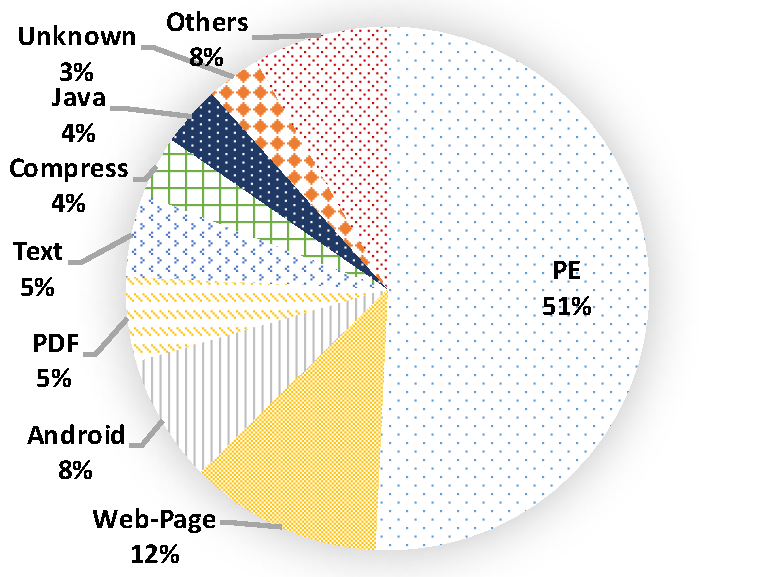
\includegraphics[width=2.in]{figure/type}
\caption{File type distributions.
%{\footnotesize{
(File types and their distributions for all VirusTotal submissions from 05/07/2016 to 09/06/2016.)
%}
}
\label{fig:type}
\end{center}
%\vspace{-0.25in}
\end{figure}


Figure~\ref{fig:type} shows the file type distribution for all submissions. 
Among all file types, Windows \textit{Portable Executable} ({\em \pe}) files, or ``Win32EXE'' and ``Win32DLL'' files, 
are the most frequently submitted type,
accounting for 51\% of all submissions.
%which conforms with a previous study~\cite{SongAPsys2016}.
Web pages and malwares on Android account for the second and third largest submissions, 
with 12\% and 8\% of all submissions respectively. 
Other popular file types include PDF, Text, compressed files, and Java files. 

Since PE files are the most common type,
we focus our study in this paper on \pe\ files 
and leave studies on other types of malwares for future. 
%If the type field for a submission is either ``Win32EXE'' or ``Win32DLL'', 
%we consider the submission is a PE file. 
In total, we collected 76 million \pe\ submissions.

\subsection{Basic Analysis}
After collecting data, we first conducted a set of basic analysis 
to learn the 



\begin{figure}[t!]
\begin{center}
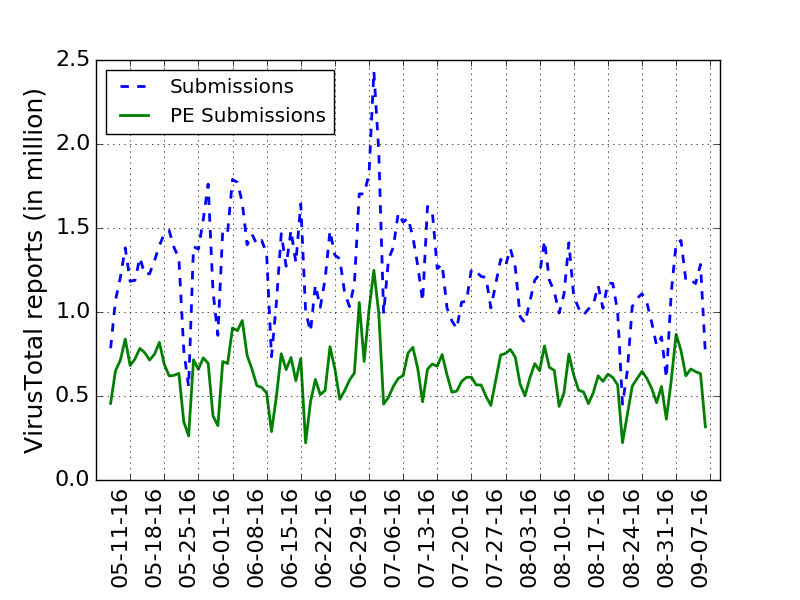
\includegraphics[width=2in]{figure/Submissions}
\caption{The number of files and PE files.
%{\footnotesize{
(The number of suspicious files and the number of PE files submitted to VirusTotal from 05/07/2016 to 09/06/2016.)
%}
}
\label{fig:subnum}
\end{center}
%\vspace{-0.25in}
\end{figure}

\begin{figure}[t!]
\begin{center}
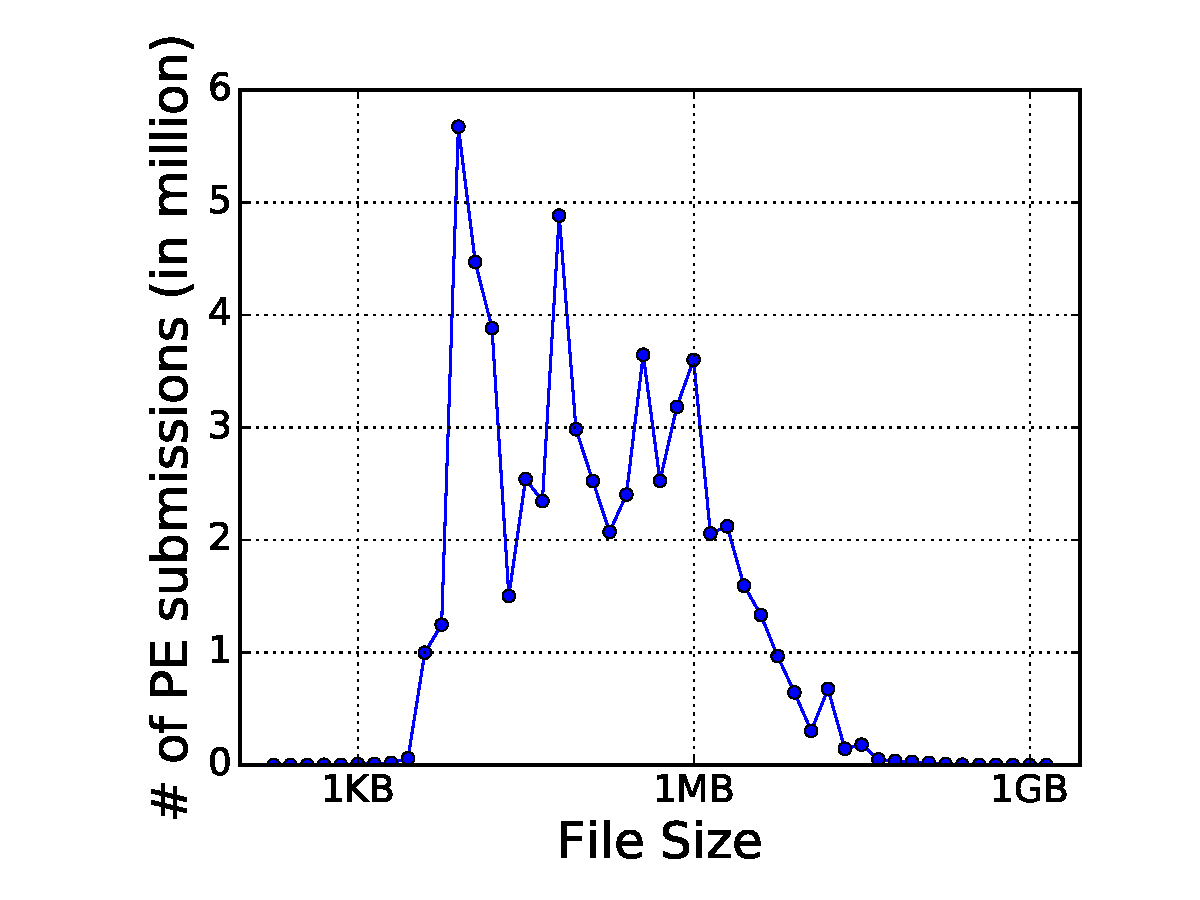
\includegraphics[width=2.5in]{figure/pesize}
\mycaption{fig:pesize}{File size distribution for PE submissions.}
{\footnotesize{(How file size distributes among all PE submissions we collect. 
Results from log2 are rounded up to nearest 0.5.)}}
\end{center}
%\vspace{-0.25in}
\end{figure}
\noindent{\bf Submission temporal, geo-location, and size distribution.} 
Figure~\ref{fig:subnum} plots the number of submissions of all types and the number of \pe\ submissions per day 
over the whole collection period.
There are a large amount of submissions every day
and the amount of submissions is fairly stable over the whole collection period.
The same conclusion can be made to \pe\ submissions.

\yiying{we still need the country distribution}

Figure~\ref{fig:pesize} shows the file size distribution for PE submissions. 
The smallest PE file is only xxx bytes, and the largest one is more than xxx\,MB. 
xxx\% of PE file fall into the range from xx\,KB to xx\,MB. 

\begin{figure}[t!]
\begin{center}
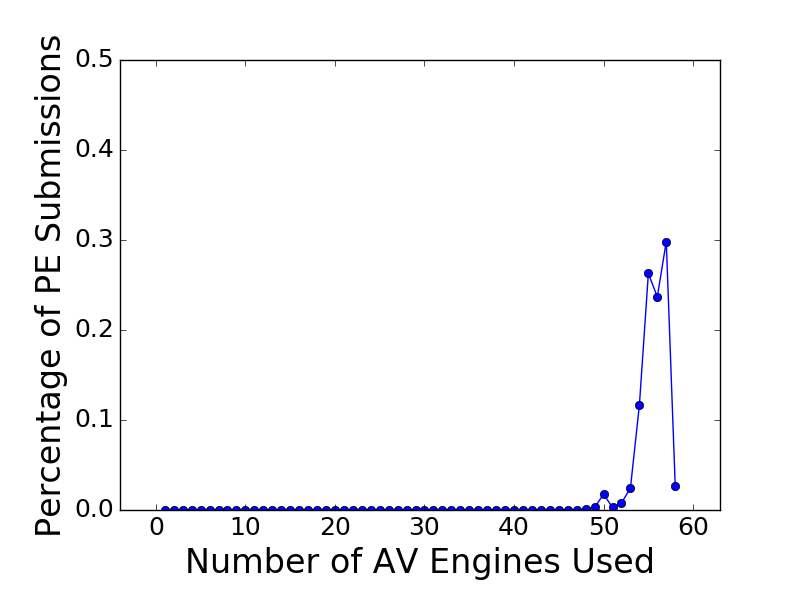
\includegraphics[width=2in]{figure/numVendor}
\caption{The distribution for the number of used anti-virus engines.
(How the number of applied anti-virus engines distributes among all PE submissions.
)
}
\label{fig:vendornum}

\end{center}
%\vspace{-0.25in}
\end{figure}
\begin{figure}[t!]
\begin{center}
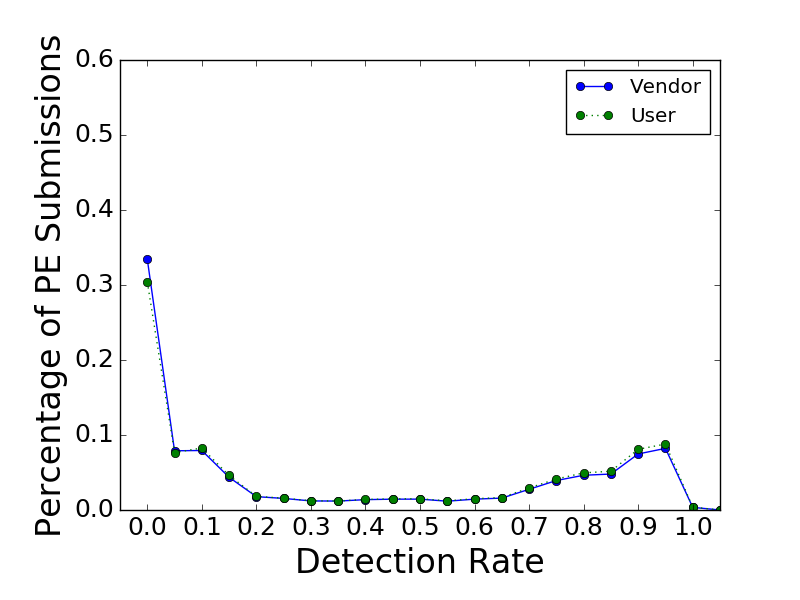
\includegraphics[width=2in]{figure/DetectionRate}
\caption{The distribution for detection rate.
(How detection rate distributes among all PE submissions. 
Each detection rate is rounded up to nearest 0.05.)
}
\label{fig:detectiorate}
\end{center}
%\vspace{-0.25in}
\end{figure}
\noindent{\textit{\underline{Anti-virus engines and detection basic analysis.}}}
%As shown in Table~\ref{tab:fields}, 
%total field is to represent the number of used anti-virus engines. 
Figure~\ref{fig:vendornum} shows the distribution for the number of used anti-virus engines. 
More than 99\% of PE submissions are analyzed by at least 50 anti-virus engines. 
Some anti-virus engines will label a submitted PE file as malware, 
while others will not. 
Positives field in Table~\ref{tab:fields} represents the number of anti-virus engines labeling the submission as malwares. 

$$ \textrm{\textit{Detection Rate}} = \dfrac{positives}{total + 1}$$

Detection rate represents the percentage of engines labeling the submission as malware. 
Adding one to total is to avoid dividing 0 exception, and more importantly, 
to give submissions labeled as malwares by more engines higher detection rate. 
For example, after adding one, submissions analyzed by 50 engines and detected by 50 engines will have a higher detection rate 
than submissions analyzed by 1 engine and detected by 1 engine. 
This formula shares the same intuition from previous work~\cite{GuoICSE2010}, when computing reputations for bug reporters. 
A larger detection rate usually indicates a more malicious malware suggested by analyzed anti-virus engines. 
Figure~\ref{fig:detectiorate} shows how detection rate distributes among all PE submissions. 

One PE file could be submitted more than once to VirusTotal. 
There are 6.72\% PE files submitted more than once to VirusTotal. 
On average, each PE file is submitted 1.19 times. 
Some anti-virus engines may produce different detection results when analyzing the same file for different submissions.
We assume there is influence among different anti-virus vendors, 
and this influence is a very important reason causing engines to change their results.
We will discuss how we model this influence and how to predict possible detection result change by using our model in Section~\ref{sec:influ}.

\subsection{Threats to validity}
\yiying{I don't know what to call this paragraph. But it should go into a subsection}

{\color{red} Another possible section name is Caveats}

Like all other empirical study works, 
our findings and conclusions need to be considered with our methodology in mind. 
We use distribution API to download submissions' metadata from VirusTotal. 
There is no guarantee that all data can be successfully downloaded. 
It could be possible that some files are submitted to VirusTotal, 
but we fail to get their information from VirusTotal.
Although we have collected huge amount of malware information from VirusTotal,
we do believe that there are malwares never submitted to VirusTotal, 
or submitted to VirusTotal much later than they appear in the real world. 
However, there are no conceivable ways to study them.
We believe the 4-month malware information we collect can serve as a representative sample for malwares in the real world. 

\section{Literature Review - How Researchers Use VirusTotal}

In this section, we introduce our findings of how current researchers make use of \vt. We collected 102 conference papers by searching \vt\ in Google Scholar. They come from many conferences include Usenix Security, NDSS, S\&P, etc. The number of papers from each conference is listed in Figure~(ref). The papers cover a large range of topics. Many of them are related to the detection or techniques of malwares, such as Android apps \cite{arp2014drebin,huangvt2016bigdata}, ransomware \cite{kharraz2016unveil} and Flash \cite{ford2009analyzing}. They mainly use \vt's detection results as baseline or ground truth. There are 89 papers use \vt\ to label or collect data set among the 102 papers. The rest 13 papers mention \vt\ for other purposes. 

There several issues that researchers need to consider in using the results. 
First, researchers could collect detection results from multiple vendors. 
It is necessary to aggregate the results into one as the label of malware or benign for some works. We would like to know how researchers aggregate them. 
Second, the detection results could change over time and it is more reliable to collect the results from \vt\ during a period of time. We would also like to know the practice on collecting results from \vt\ over time. 
Thrid, vendors could have different impacts. It is also interesting to know whether and how researchers considered the different impacts of vendors.

%Last but not least, it is worth considering how we merge results from different vendors. 
First, we look at how researchers merge detection results. In most cases, researchers get results from more than 40 or 50 vendors and merge the results as one for their dataset. 
There are mainly two ways of merging: 1) considering a submission as malicious if any vendor can detect; 2) considering a ratio or a threshold for the number of vendors. 
For instance, 
Among the 89 papers, 26 papers (29.2\%) use the first way and 46 papers  (51.7\%) use the second way. The rest 17 papers (19.1\%) do not mention how they merge results from different vendors.

Second, there are only 4 papers consider that the detection results could change over time, and collect the results from \vt\ during a period of time. The length of time could vary from several days \cite{kharraz2016unveil, rajab2013camp} to months \cite{neeles, wressnegger2017looking}. 

Third, among the 89 papers, only 8 consider that different vendors shall have different impact. Most of them pick out three to more than ten vendors to discuss their impact, because of their influence in industry or good performance on detection rate. For instance, Arp et al. \cite{arp2014drebin} inspected the output of ten vendors and list their detection rate anonymously. In addition, all of the papers treat the vendors equally. %Thomas et al. \cite{thomas2015ad} listed detection rate of 3 vendors. 

%“we send each sample to the VirusTotal service and inspect the output of ten common anti-virus scanners (AntiVir, AVG, BitDefender, ClamAV, ESET, F-Secure, Kaspersky, McAfee, Panda, Sophos)
%” from a NDSS paper (index 14)


%They collected  Kharraz et al. \cite{kharraz2016unveil} Graziano et al. \cite{neeles} Rajab et al. \cite{rajab2013camp} and Wressnegger et al. \cite{wressnegger2017looking}.





\section{Basic Properties}
\label{sec:basic}

After collecting data, we first conducted a set of analysis 
to learn various basic properties of submission files, 
submission sources, and anti-virus engines.
These properties give an overview of how real-world submissions and anti-virus engines are like
and serve as the foundation for our more advanced analysis in the next two sections. 





%\noindent{\textit{\underline{Submission temporal, geo-location, and size distribution.}}}

\subsection{Submission Temporal, Geo-location, and Size Distribution}
\label{sec:basicanal}


\begin{figure}[t!]
\begin{center}
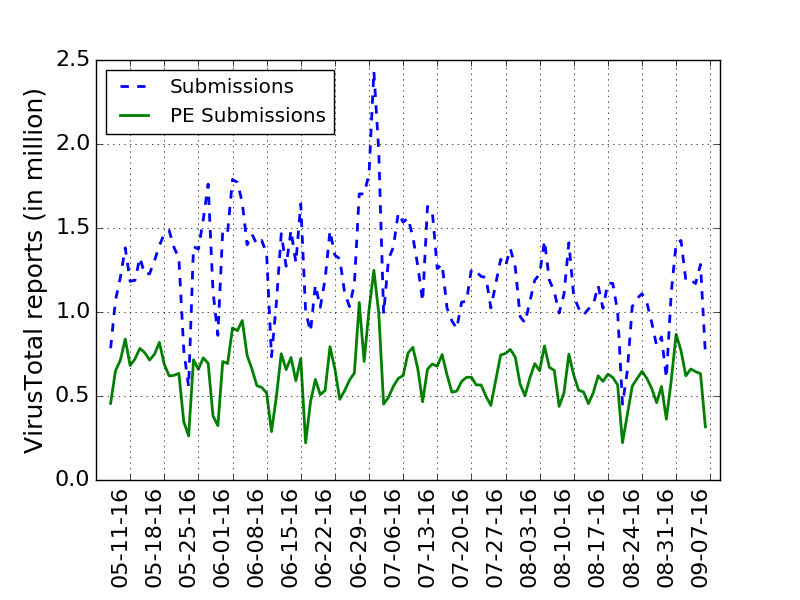
\includegraphics[width=2in]{figure/Submissions}
\caption{The number of files and PE files.
%{\footnotesize{
(The number of suspicious files and the number of PE files submitted to VirusTotal from 05/07/2016 to 09/06/2016.)
%}
}
\label{fig:subnum}
\end{center}
%\vspace{-0.25in}
\end{figure}


Figure~\ref{fig:subnum} plots the number of submissions of all types and the number of \pe\ submissions per day 
over the whole collection period.
There are a large amount of submissions every day
and the amount of submissions is fairly stable over the whole collection period.
The same conclusion can be made to \pe\ submissions.

One PE file could be submitted more than once to VirusTotal. 
On average, each PE file was submitted 1.19 times and 6.72\% PE files were submitted more than once. 

\begin{figure}[t!]
\begin{center}
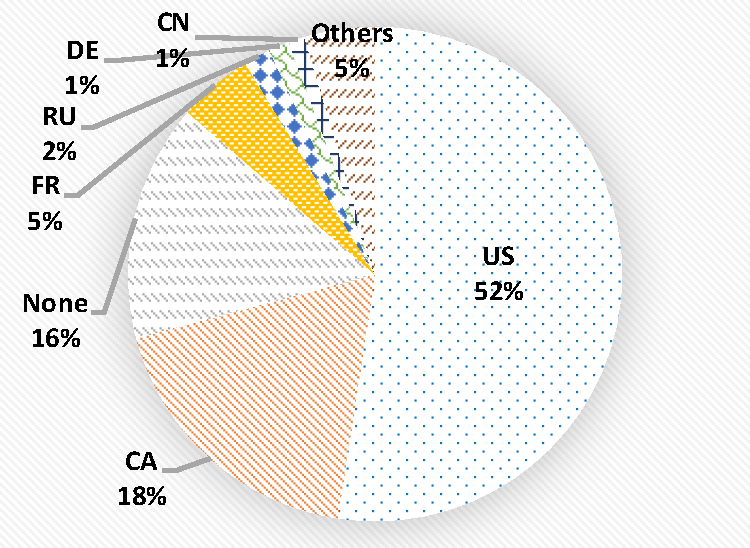
\includegraphics[width=2in]{figure/countryPie}
\caption{How PE submissions distribute among different countries.
%\footnotesize{
(Only countries with more than 1\% PE submissions are shown.)
%}
}
\label{fig:countryPie}
\end{center}
%\vspace{-0.25in}
\end{figure}

For around 16\% of PE submission, 
\vt\ fails to provide their source country information. 
All other submissions are conducted from 221 countries. 
The top 6 countries in PE submission number are US, Canada, France, Russia, Germany, and China, 
as shown in Figure~\ref{fig:countryPie}.

\begin{figure}[t!]
\begin{center}
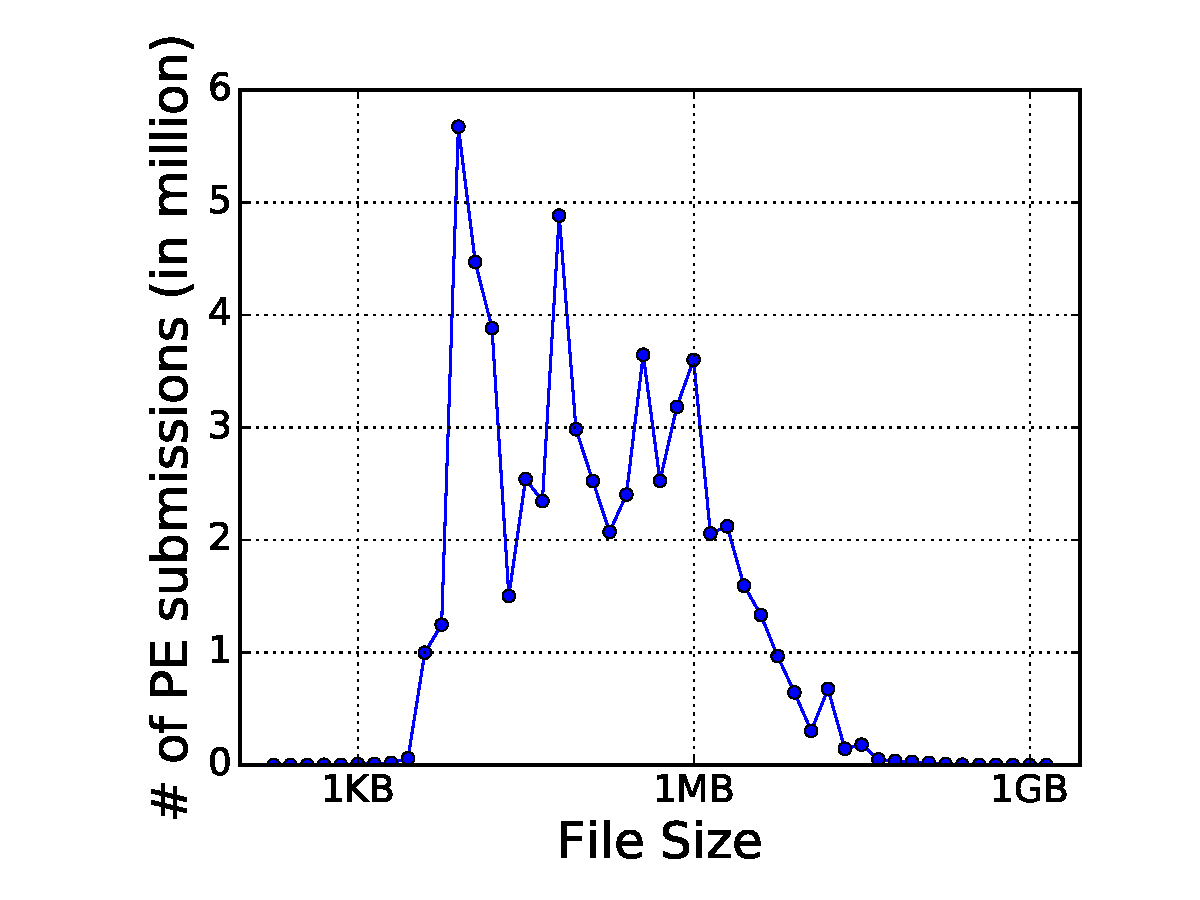
\includegraphics[width=2.5in]{figure/pesize}
\mycaption{fig:pesize}{File size distribution for PE submissions.}
{\footnotesize{(How file size distributes among all PE submissions we collect. 
Results from log2 are rounded up to nearest 0.5.)}}
\end{center}
%\vspace{-0.25in}
\end{figure}

Figure~\ref{fig:pesize} shows the file size distribution for \pe\ submissions. 
The smallest \pe\ file is only 187 bytes, and the largest one is more than 1\,GB. 
99.58\% of PE file fall into the range from 4\,KB to 32\,MB. 

{\bf Observation 1:} 
{\em \vt\ constantly receives large amount of submissions from all over the world. 
Most submitted files have small to middle sizes and are only submitted once, 
but some files are submitted many times.}

%\noindent{\textit{\underline{Submission sources.}}}
\subsection{Source ID}
\label{sec:source_id}

\begin{figure}[t!]
\begin{center}
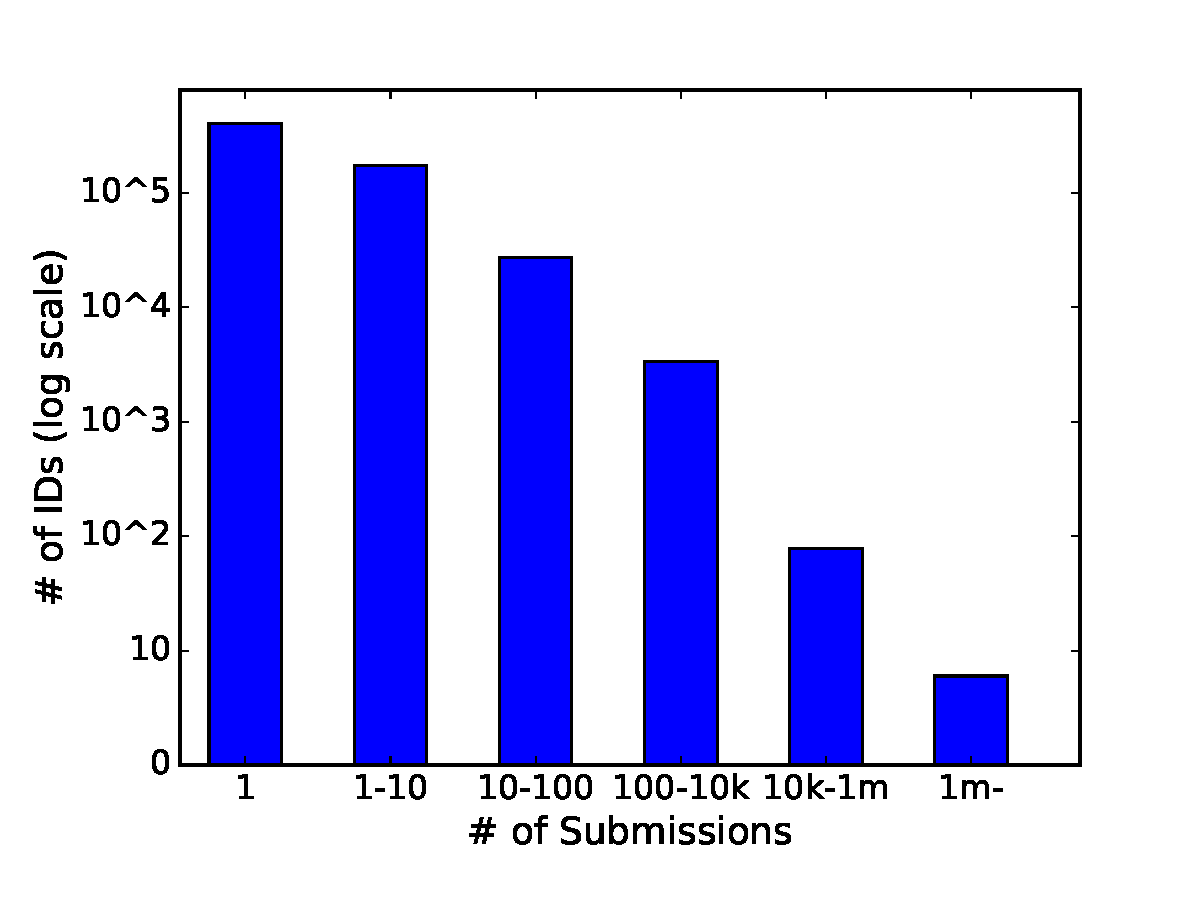
\includegraphics[width=2.5in]{figure/IDDistribution}
\mycaption{fig:iddis}{The distribution for source ids.}
{\footnotesize{(How source ids distribute among all source id groups. 
We divide groups based on PE submissions made by each source id.)}}
\end{center}
%\vspace{-0.25in}
\end{figure}

Both normal users and anti-virus vendors use \vt\ to detect malwares or evaluate products.
Usually, vendors tend to make more submissions than normal users, since they need to test their products on many files.
Thus, we use the number of submissions to measure what type of users a source ID is.

We separate the number of submissions into six categories:
one submission, one to ten submissions, ten to 100 submissions, 100 to 10000 submissions, 10000 to 1 million submissions, and larger than 1 million submissions.
Figure~\ref{fig:iddis} plots the number of source IDs in log scale in the first five categories.
There are only 6 source IDs that have more than 1 million submissions and we suspect that these IDs are either bogus or robots 
that constantly make submissions to \vt.
For the rest, we find that the number of source IDs dramatically drops when the number of submissions is more than 100.
Thus, we categorize the source IDs as normal user if they have less than 100 submissions and as vendors if they have more than 100 submissions.

{\bf Observation 2:} 
{\em Most \vt\ users are normal users that make occasional submissions, while a small set of anti-virus vendors use \vt\ and make a huge amount of submissions.}


%\noindent{\textit{\underline{Anti-virus engines and detection basic analysis.}}}

\subsection{Anti-virus Engines}

\begin{figure}[t!]
\begin{center}
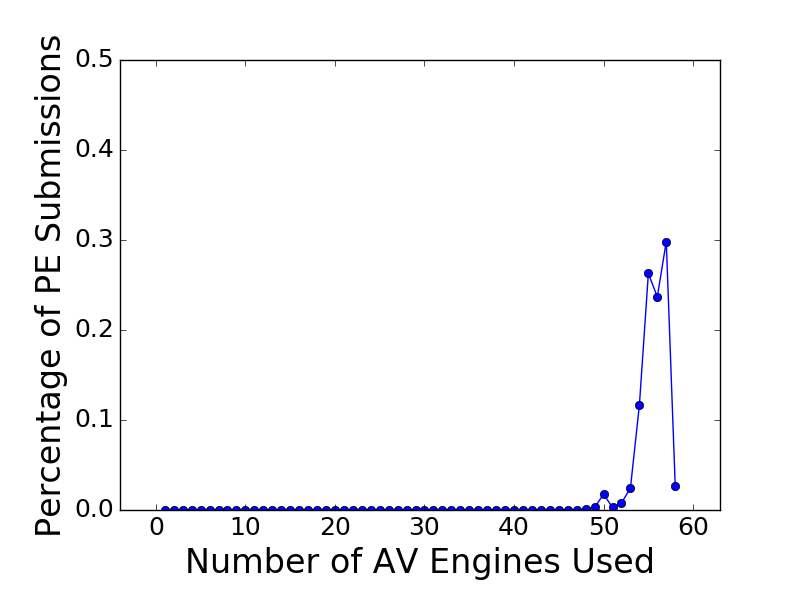
\includegraphics[width=2in]{figure/numVendor}
\caption{The distribution for the number of used anti-virus engines.
(How the number of applied anti-virus engines distributes among all PE submissions.
)
}
\label{fig:vendornum}

\end{center}
%\vspace{-0.25in}
\end{figure}
\begin{figure}[t!]
\begin{center}
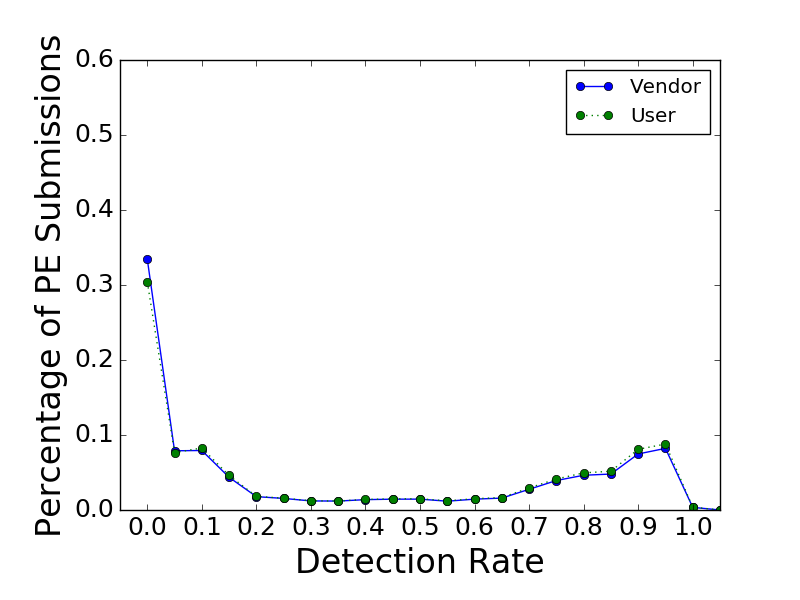
\includegraphics[width=2in]{figure/DetectionRate}
\caption{The distribution for detection rate.
(How detection rate distributes among all PE submissions. 
Each detection rate is rounded up to nearest 0.05.)
}
\label{fig:detectiorate}
\end{center}
%\vspace{-0.25in}
\end{figure}


After learning the basic properties of submissions and source IDs, 
we now move to the basic analysis of anti-virus engines and their detection of malware.
Figure~\ref{fig:vendornum} shows the distribution of the number of anti-virus engines used by \vt\ on each submission. 
More than 99\% of PE submissions are analyzed by at least 50 anti-virus engines. 
We suspect that \vt\ sets some threshold when running anti-virus engines and 
will abort an engine when it takes too long to run on a submission,
causing few submissions having fewer than 50 engines.

For the same submission, different anti-virus engines can make different detection results, \ie, 
some mark the submission as malware while others don't.
To quantify the detection results of a submission,
we use a value we call {\em Detection Rate}.
Detection rate represents the percentage of engines labeling the submission as malware. 

$$ \textrm{\textit{Detection Rate}} = \dfrac{positives}{total + 1}$$

We add one to {\bf total} to avoid divide-by-zero exception, and more importantly, 
to have higher detection rate to submissions labeled as malwares by more engines.
For example, submissions analyzed by 50 engines and detected by 50 engines 
has a higher detection rate 
than submissions analyzed by one engine and detected by one engine. 
%This formula shares the same intuition from previous work~\cite{GuoICSE2010}, when computing reputations for bug reporters. 
%A larger detection rate usually indicates a more malicious malware suggested by analyzed anti-virus engines. 

Figure~\ref{fig:detectiorate} shows the distribution of detection rates over all \pe\ submissions.
We separately consider submissions made by normal users and by anti-virus vendors 
(as defined in Section~\ref{sec:source_id}).
Interestingly, overall most submissions to \vt\ are likely to be benign files, \ie, has low detection rate.
Around half of the submissions were labeled as benign by all engines (a detection rate of zero),
and only 31.5\% submissions were labeled as malware by at least half of the engines.
Surprisingly, the detection rates of submissions made by normal user and by anti-virus vendors are very similar.
One probable explanation is that anti-virus vendors obtain their suspicious files 
from end users and thus have similar behavior as normal users' submissions.
Another possible reason is that as suspicious files are announced publicly, 
both normal users and vendors will try to test them with \vt.



{\bf Observation 3:} 
{\em Most submissions to \vt\ are labeled as benign and 
submissions made by normal user and by anti-virus vendors have similar probabilities of being labeled as malware.}



\section{Correlation between Submission Properties and Detection Rate}
\label{sec:corr}
This section presents our study of the correlation between various properties of
\pe\ submissions and their detection rate. 
Detection rate is what most \vt\ users refer to decide whether their submissions
are benign or malware and the first thing that a user of \vt\ uses. 
Therefore, it is important to study what factors affect or correlate to detection rates. 
We focus on \vt\ submissions' properties, which can be obtained without executable binary files and more lightweight than static features.
The results provide a lightweight mechanism to guide security researchers 
and vendors to have targeted investigation over
{\em suspicious} files, 
files that have the factors that we identify as highly correlated to detection rate.

We studied a range of properties and their correlation with detection rate
and found that three factors have higher correlation:
submission file size,
historical submission properties, and the reputation of source IDs.
We also built a regression model based on these three factors to predict detection rate.
We present these correlation study results and our regression model in this section.
In the next section, we will present our further analysis of what can affect the detection result of anti-virus engines
and if detection rate is a perfect measurement of the likelihood of malware.


\begin{figure}[t!]
\begin{center}
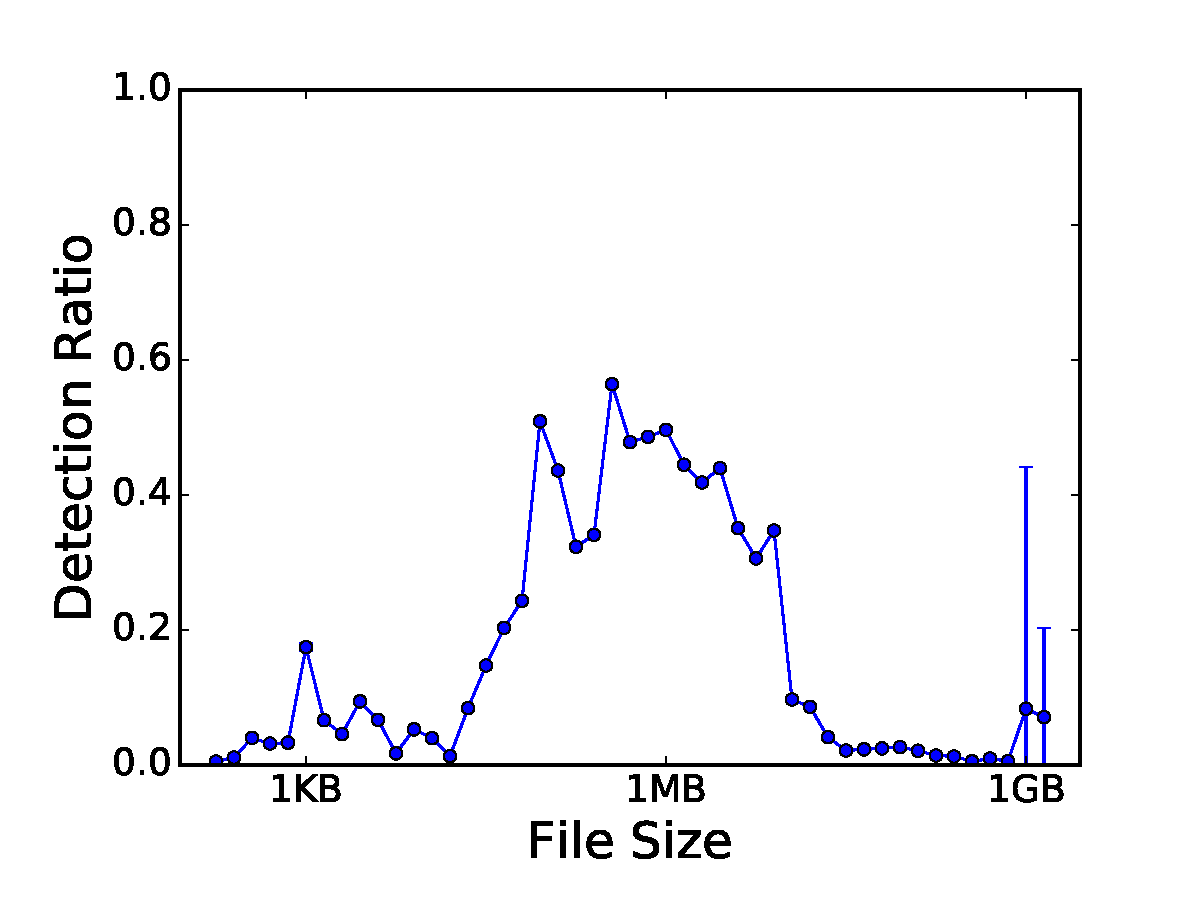
\includegraphics[width=2in]{figure/size}
  \caption{How detection rate changes with file size.
(
95\% confidence interval is also drawn for each point.
Results of log2 for the original file sizes are rounded to the nearest 0.5 value.)
}
\label{fig:size}
\end{center}
%\vspace{-0.25in}
\end{figure}


\subsection{File Size}
\label{sec:size}
Anecdotally, \pe\ malwares are most likely to have small to medium size. 
To verify this, we analyzed the relationship between submission file size and detection rate. 
Figure~\ref{fig:size} presents the average detection rate and 
the 95\% confidence interval for different file sizes.
A wider confidence interval implies that
the calculated average detection rate is farther away from the real average detection rate.
We use discrete file sizes of powers of two in our analysis and in this graph,
i.e., we calculate the log2 of each original file size and round it to the nearest 0.5 value.
Overall, we find that files with size from 90KB to 4MB have higher detection rate, more than 20\% on average. 
Except for the last two points which represent a small amount of files that are bigger than 1GB, 
all other sizes have high confidence.   

{\bf Observation 4:} 
{\em \pe\ malwares are mostly likely to have small to medium size.}

An immediate question to raise is whether the high detection rate of files with small to medium size
is because these files also contribute to most of the submissions as shown in Figure~\ref{fig:pesize}.
As we will discuss in Section~\ref{sec:history}, the correlation of submissions and detection rate is more complex and non-linear.
Thus, there is a more fundamental reason behind the file size correlation with detection rate.
One likely reason of this correlation is that files that are too small are not enough to express the
malware functions while files that are too big are difficult to spread.

\subsection{Submission History}
\label{sec:history}




\begin{figure}[t!]
\begin{center}
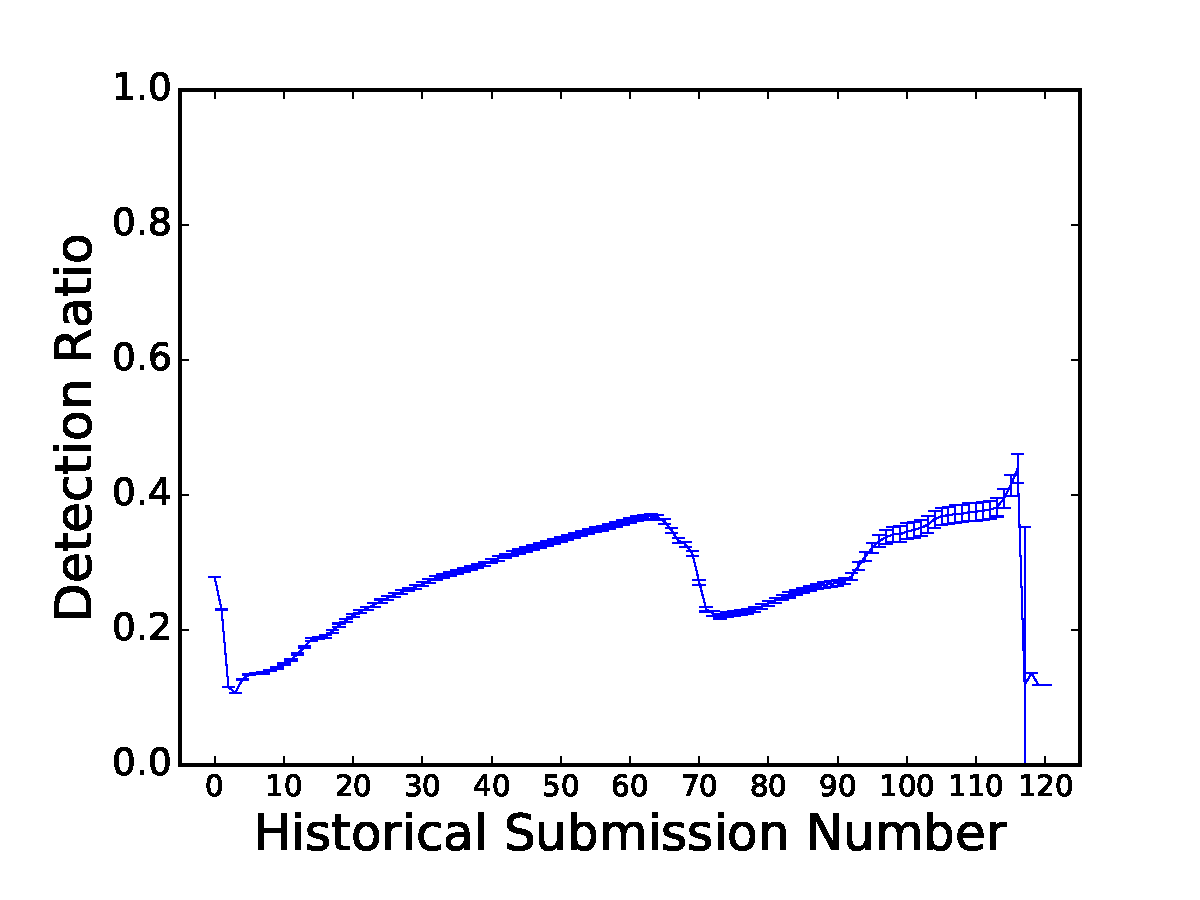
\includegraphics[width=2in]{figure/SubNum}
\caption{
The relation between historical submission number and detection rate.
(
How detection rate changes with historical submission number. 
Each historical submission number is rounded up to nearest 5.
95\% confidence interval is also drawn for each point.
)	
}
\label{fig:hisnum}
\end{center}
%\vspace{-0.25in}
\end{figure}

%\begin{figure}[t!]
%\begin{center}
%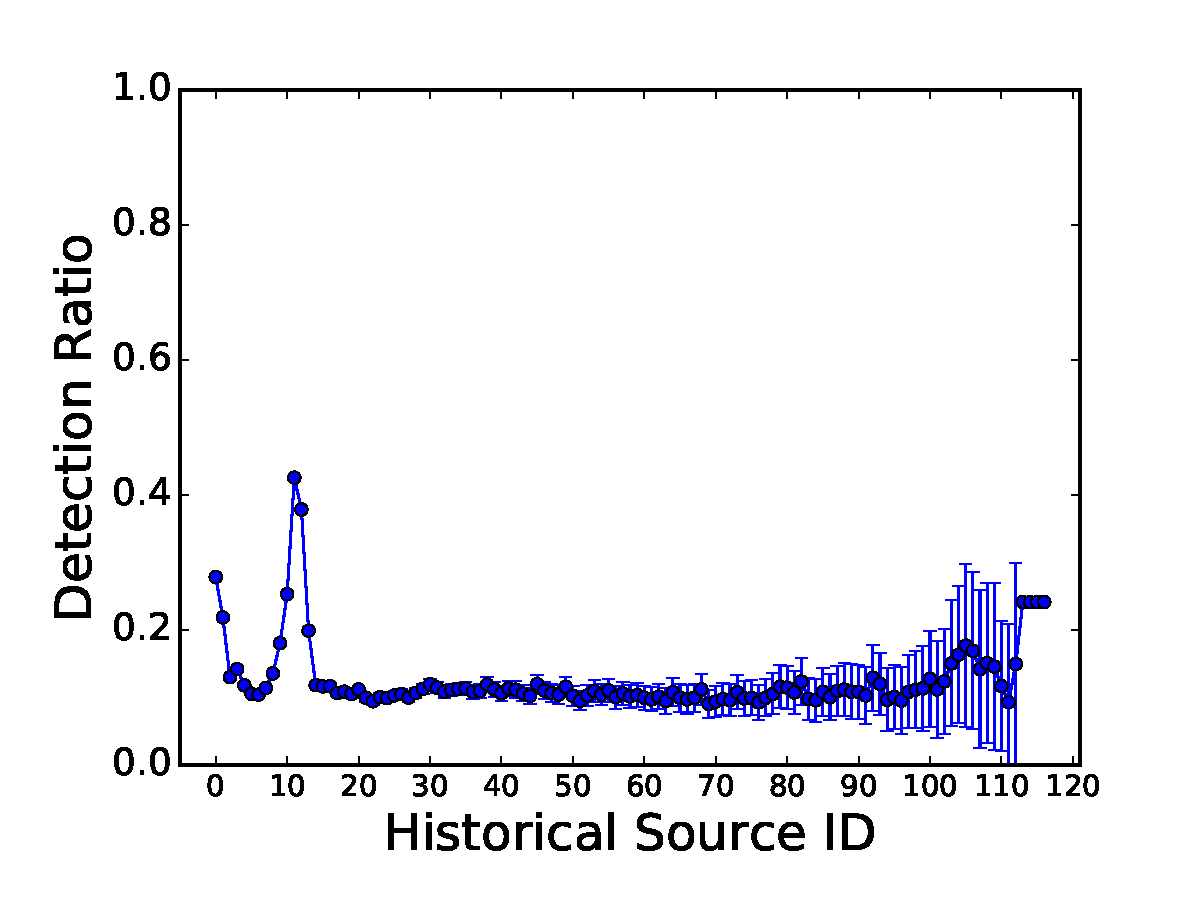
\includegraphics[width=2.5in]{figure/SubID}
%  \mycaption{fig:hisid}{The relation between the number of historical source ids and detection rate.}
%{\footnotesize{(How detection rate changes with the number of historical source ids. 
%Each historical number of source ids is rounded up to nearest 5.
%95\% confidence interval is also drawn for each point.)}}

%\end{center}
%\vspace{-0.25in}
%\end{figure}


As discussed in Section~\ref{sec:basicanal}, there are files that have been submitted more than once to VirusTotal. 
It is worthwhile to investigate this {\em history of submission} and how history affects future.
We study the correlation between submission history and the detection rate of the current submission.
Among the different types of historical information that we study,
we find that the number of submissions made in history has higher correlation to detection rate.

%\noindent{\textit{\underline{The number of submissions in history.}}}
To study the submission history, we first sort all submissions for each file chronologically
and then collect the number of all submissions made before submission $s$ for each submission $s$ in \vt.
Next, we calculate the correlation between detection rate and the number of submission in history.
Figure~\ref{fig:hisnum} plots how detection rates change over the number of historical submissions.
Interestingly, there are two main ranges that steadily increase and there are three drops in the beginning, middle, and end.

To explain this effect, we first look at the two factors that can both influence detection rates:
the percentage of benign files submitted and the amount of anti-virus engines labeling the submission as malware.
%Two factors can influence detection rates and explain the above effect.
Obviously, with more benign files submitted, detection rate will decrease
and with more engines labeling malwares, detection rate will increase. 
In the the two stages of detection rate increasing, 
with more submissions, more engines are able to identify malwares 
and the increase of percentage of engines identifying submitted malwares dominates. 
In the range that detection rate drops, 
VirusTotal users stop submitting files that have already been identified as malwares,
and the increase of percentage of benign files submitted to VirusTotal dominates. 



{\bf Observation 5:} 
{\em The number of submissions made in history has correlation with detection rate, but the correlation is non-linear and is affected by multiple factors.}


\subsection{Reputation of Source ID}
\label{sec:reputation}



\begin{figure}[t!]
\begin{center}
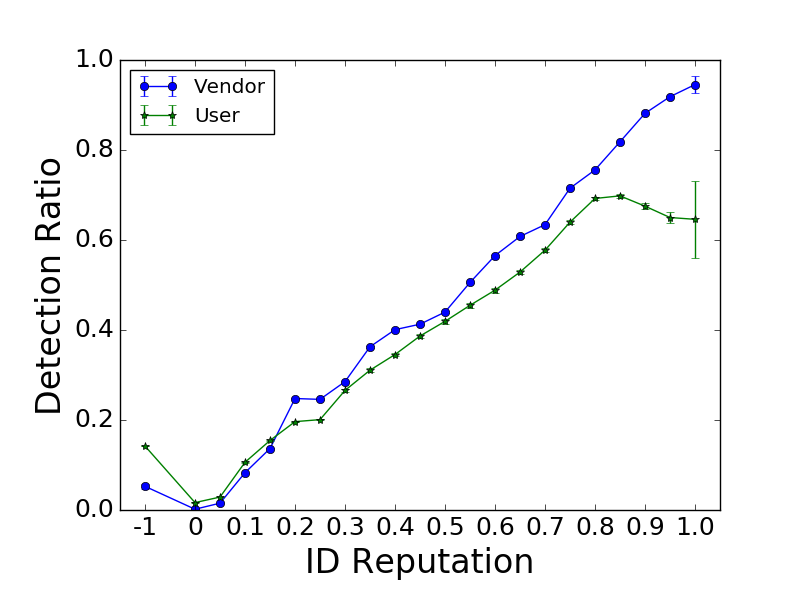
\includegraphics[width=2in]{figure/IDReputation}
\caption{The relation between source id's previous reputation and detection rate.
(How detection rate changes with the value of source id's reputation. 
Each reputation is rounded up to nearest 0.05.
Reputation -1 means the source id did not make any submission before. 
95\% confidence interval is also drawn 
for each point.)
}
\label{fig:idreputation}
\end{center}
%\vspace{-0.25in}
\end{figure}

Different users of online services such as \vt\ often have different {\em reputation} 
because of different motivations, objectives, and backgrounds.
For example, some users can randomly trying out \vt\ with no specific objective and thus submit random files,
while other users have clear goals and motivations and thus only submit suspicious files.
The rationale behind reputation is that \vt{} users would have a roughly constant submission pattern, 
and it is promising to use their historical submission to predict their future submission.
Previous work~\cite{GuoICSE2010} reported that there is a correlation between bug reporter's reputation and the likelihood for the bug being fixed. 
We also observe correlation between the reputation of source ID and submission's detection rate. 

Intuitively, a user that have submitted more files that were detected as malware suggest 
that she is more likely to use \vt\ to detect malware in suspicious files 
and thus should be given higher reputation.
To quantify this, we define the reputation of a source ID as the follow.
The reputation of a source ID is not a fixed value and can change over time. 

%\theoremstyle{definition}
\begin{definition}{Reputation:}
Given a submission $S$ with source ID $N$, 
we define the reputation of $N$ when conducting the submission $S$ as the average detection rate for all submissions conducted by $N$ before $S$. 
If $N$ did not make any submission before, we define the reputation to be $-1$. 
\end{definition}

Before conducting our source ID reputation analysis, we first filter out submissions
without source ID information, and submissions by source ID with more than 1 million submissions (bogus or robots).
To calculate source ID reputation, we first sort all submissions from the same source ID chronologically, 
and calculate reputation for each source id when conducting each submission. 
We further separate normal users from vendors and analyze the correlation of their ID reputation and detection rate.

Figure~\ref{fig:idreputation} plots the average detection rate and the 95\% confidence interval 
as the source ID reputation increases for normal users and for anti-virus vendors.
We round up reputation values to their nearest 0.05 values. 

Detection rate steadily increase as the reputation increases from 0 to 1 for vendors and from 0 to 0.8 for normal users.
Except the points when reputation is 1, all other results have high confidence.
Interestingly, for both normal user and vendors the detection rate with reputation -1 is higher than with reputation 0,
which means that the first submissions conducted by all source IDs (reputation -1) 
are overall have higher detection rate than 
the submissions conducted by IDs that have only submitted benign files (reputation 0).

For normal users, the detection rate drops when reputation is greater than 0.8.
This means that for normal users, it is difficult for them to always submit suspicious files detected by almost all vendors.
Vendors do not have this behavior and their detection rate always increases with higher reputation (other than reputation -1).


{\bf Observation 6:} 
{\em There is a high correlation between user reputation and detection rate of their submissions for both normal users and anti-virus vendors.}


\subsection{Regression Model}

We build a linear regression model to predict the detection rate for a submission, 
by using factors we discussed above.  
We filter submissions without source ID reputation information, as we discussed in Section~\ref{sec:reputation}. 
We then randomly divide remaining submissions into training set and testing set with equal size. 
We choose random guess as baseline model, 
which is to guess the detection rate for any submission 
as the mean of detection rate for all training submissions. 
We calculate the mean absolute error (mae)~\cite{mae} 
and the mean squared error (mse)~\cite{mse} to compare our regression model and baseline model. 

For in sample testing, mae and mse for our regression model are 0.2227 and 0.0718 respectively, 
while for baseline model they are 0.3345 and 0.1327. 
For out of sample testing, mae and mse for our regression model is 0.2223 and 0.0716 respectively, 
and they are 0.3342 and 0.1325 for baseline model. 
For both in sample testing and out of sample testing, our regression model can beat baseline model significantly. 


{\bf Observation 7:} 
{\em Regression model based on studied factors can help the prediction of detection rate for malware submissions.}


\subsection{Discussion}


From our analysis, file size, number of submissions in history, 
and source ID reputation are all highly correlated with detection rate.
Our regression model based on these three factors can effectively help predict detection rate for \vt\ submissions, and this also verifies our correlation studying results. 
All the three studied factors can be obtained without analyzing binary executable files.
These factors plus our regression model provide a lightweight estimation or prediction for future submissions.  
Doing so can help reduce researchers' and vendors' effort to focus on more interesting files---files that are more likely to be malicious.
Anti-virus vendors can also inspect results which are variant from our prediction results 
to identify possible false positives or false negatives in their products. 
File size information can be accessed in \vt~'metadata. 
Number of submissions in history and source ID reputation are computed by ourselves. 
Our studying results suggest that \vt should also track number of submissions in history for each file and reputation for each source ID in the future. 


\section{Influence Among Anti-Virus Engines}
\label{sec:influ}

Anti-virus vendors frequently use VirusTotal to identify false negatives in their products, 
which are malware they fail to detect but detected by other vendors~\cite{vt-usage}.
As discussed in Section~\ref{sec:meth}, many files are submitted to VirusTotal more than once, 
and more than 99\% submissions are analyzed by at least 50 anti-virus engines. 
Interestingly, we observe that some engines fail to identify some malware during early submissions, 
but they catch up when analyzing later submissions.

This observation led us to ask one important question that have never been studied before:
{\em is there influence across different anti-virus vendors?}
That is, can an anti-virus vendor's decision be affected by other vendors' malware detection results?
With the large number of anti-virus engines in the wild, it is important to understand if an anti-virus engine is
reliable and can be trusted.  

This section presents our answer to this question by quantifying the influence across anti-virus engines.
Specifically, we study the historical submissions of a file and
how anti-virus engines change their labels of the same file over time.
We also provide a prediction model on whether an engine will identify a file as malware in the future
after labeling the file as benign---a warning flag that this engine's decision is highly likely to be resulted from the influence of other engines.

\subsection{Influence Graph}
\label{sec:model}
We now discuss our proposed mechanism to analyze the influence among anti-virus engines.
Our goal is to estimate the {\em trustworthiness} of an anti-virus engine $i$, $T_i$.

We propose to model the anti-virus engine influence problem as a graph problem.
Influence propagation in social networks is a well-studied topic in the web mining area. 
Inspired by social graph solutions~\cite{Influence}, we propose to use graphs to represent the relationship between vendors 
and model influence among different vendors based on static models.
% first overview static models in our usage scenario,
%and then we discuss how we evaluate static models on data we collect. 

We first build a complete directed graph $G = (V, E)$ called {\em influence graph} for the influence problem, 
where the nodes $V$ are vendors and edges model the likelihood of influence between two vendors. 
We choose to use a complete graph because we initially assume that it is possible to have influence from one vendor to any other vendor.

We use {\em action} to describe the detection result of an engine to a submission. Since a file can be
submitted more than once and an engine can analyze it multiple times, we need to associate action with
time. We formally define an action, $a$, at time $t$ as $(u, a, t)$ or $(u, \bar{a}, t)$,
where the former represents an anti-virus engine identifies the submission as malware 
and the latter represents it identifies the submission as benign.

We limit the goal of this study to detecting whether or not a vendor changes its labeling of a file from
benign to malware because other vendor(s) have labeled it as malware (what we call {\em positive influence}). 
%This is because {\color{red} vendors detecting malware earlier are more trustworthy than vendors following others.}
Thus, we do not consider the case of changing from labeling malware to benign ({\em negative influence}). 
We also assume that after a vendor labels a file as malware it will not change its decision.
A similar model can be applied to study negative influence and we leave it for future work.

We associate each edge $(u, v) \in E$ in the graph $G$ 
with an {\em influence probability} $p_{u,v}$,
which represents the probability that after $u$ takes an action $v$ will follow $u$ to take the same action.
Since we only consider positive influence, 
when calculating $p_{u,v}$, we only consider cases where after $u$ has labeled a submission as malware, 
$v$ will change its label from benign to malware in a later time, i.e., 
$\exists$  $(u, a, t_1)$, $(v, \bar{a}, t_2)$, $(v, a, t_3)$ where $t_1<t_3$ and $t_3>t_2$. 


%\yiying{does this action include both turning from labeling benign to malware and from malware to benign? 
%does it include the first label (no prior labeling by the same node)? you need to explain what an "action" is.}
%Since the graph is a complete graph, 
%all other nodes are all $v$'s neighbors. 

To capture the engines influence an engine, we use the neighbor relationship in the influence graph. 
We define $S_v(a)$ to be the set of $v$'s neighbors that take action $a$ before $v$ in time. 
The probability that $v$ will follow its neighbors to take the same action can then be calculated as:

\begin{equation} \label{eq:setp}
%$$p_v(S_v(a)) = 1 - \prod\limits_{u \in S_v(a)}(1 - p_{u,v})$$
p_v(S_v(a)) = 1 - \prod\limits_{u \in S_v(a)}(1 - p_{u,v})
\end{equation}

We can use $p_{u,v}$ to further estimate the trustworthiness of an engine, $T_v$.
Intuitively, if an anti-virus engine gets more influence from others,
it is less reliable and trustworthy. Thus, we have

\begin{equation} \label{eq:trust}
T_v = \frac{1}{\sum\limits_{u \neq v}{p_{u,v}}}
\end{equation}


\subsection{Influence Probability Estimation Model}
\label{sec:influenceprob}
From the above analysis, we can see that the influence probability is the key of our anti-virus engine
influence problem.
After knowing the value of the influence probability $p_{u,v}$ between all engine pairs $u$ and $v$,
it is easy to calculate the trustworthiness of all engines.
The problem now boils down to estimating $p_{u,v}$.

To estimate the influence probability between two engines, we propose to use the statistics of actions taken by
an engine on a file and the action propagation between two engines. 
Specifically, we use the {\em happen-after} relationship to
define {\em action propagation}; if an action of an engine is taken after an action of another engine, we say that
this action is propagated.

To assist the definition of action propagation, we first define a few types of submission sets.
We use $A_u$ to represent the set of submissions ever identified by $u$ as malware in its history
and $\bar{A}_u$ to represent the set of submissions that have been labeled as benign and yet not labeled as malware by $u$.
%the number of actions taken by $u$, 
%or the number of malware identified by $u$. 
%\yiying{I think all these $A$ should be a collection/set, not the total number, since you use $\in$ later}
%\yiying{Verify that the above sentence is correct.}
Further, we define the set of actions taken by both $u$ and $v$ as $A_{u\&v}$ 
and the set of actions taken by either $u$ or $v$ as $A_{u|v}$.
Thus, $|A_{u|v}| =   |A_u| + |A_v| - |A_{u\&v}|$.
With these sets defined, we formally
define {\em action propagation} in the following equation 
and use $A_{u2v}$ to represent the set of all the actions that are propagated from $u$ to $v$. 

%\begin{definition}{Action Propagation:}
{Action Propagation:}
An action $a$ propagated from $u$ to $v$ iff: (i) $\exists$ $(v, \bar{a}, t_i)$ $\in$ $\bar{A}_v$ 
and $(v, a, t_k)$ $\in$ $A_v$, with $t_i < t_k$; (ii) $\exists$ $(u, a, t_j)$ $\in$ $A_u$, with $t_j < t_k$ and $u \neq v$. 
%\end{definition}

With these definitions, we now present our four proposed static models to estimate $p_{u,v}$.

{\bf Bernoulli distribution} estimates $p_{u,v}$ as the ratio of the number of actions 
propagated from $u$ to $v$ over the total number of actions taken by $u$.

$$p_{u,v} = \frac{|A_{u2v}|}{|A_u|}$$ 

{\bf Jaccard index} estimates 
$p_{u,v}$ as the number of actions propagated from $u$ to $v$ divided by 
the number of actions taken either by $u$ or by $v$.

$$p_{u,v} = \frac{|A_{u2v}|}{|A_{u|v}|}$$ 

On top of the Bernoulli distribution and the Jaccord index,
we add an additional consideration called {\em partial credit}.
When $v$ takes an action $a$, it may be influenced by the combination of all its neighbors $S_v(a)$ 
taking the action $a$ before $v$. %Partial credit takes this intuition. 
To account for this effect, we use partial credit 
and calculate the partial credit for $u$ who takes an action $a$ before $v$ as 

$$credit_{u,v}(a) = \frac{1}{|S_v(a)|}$$

{\bf Bernoulli distribution with partial credit} 
estimates $p_{u,v}$ as the sum of all partial credits taking by $u$ for actions propagated from $u$ to $v$, 
dividing by the number of actions taken by $u$. 

$$p_{u,v} = \frac{\sum\limits_{a \in A_{u2v}}{credit_{u,v}(a)}}{|A_u|}$$

{\bf Jaccard index with partial credit} 
estimates $p_{u,v}$ as the sum of all partial credits taking by $u$ for actions propagated from $u$ to $v$, 
dividing by the number of actions taken either by $u$ or by $v$. 

$$p_{u,v} = \frac{\sum\limits_{a \in A_{u2v}}{credit_{u,v}(a)}}{|A_{u|v}|}$$


Since $|A_{u|v}|$ is not less than $|A_u|$, 
$p_{u,v}$ calculated by Jaccard index is not larger than $p_{u,v}$ calculated by Bernoulli distribution. 
For Bernoulli distribution and Jaccard index, 
considering partial credit will decrease $p_{u,v}$ calculated by both of them. 

\begin{figure*}
\centering
\subfloat[]{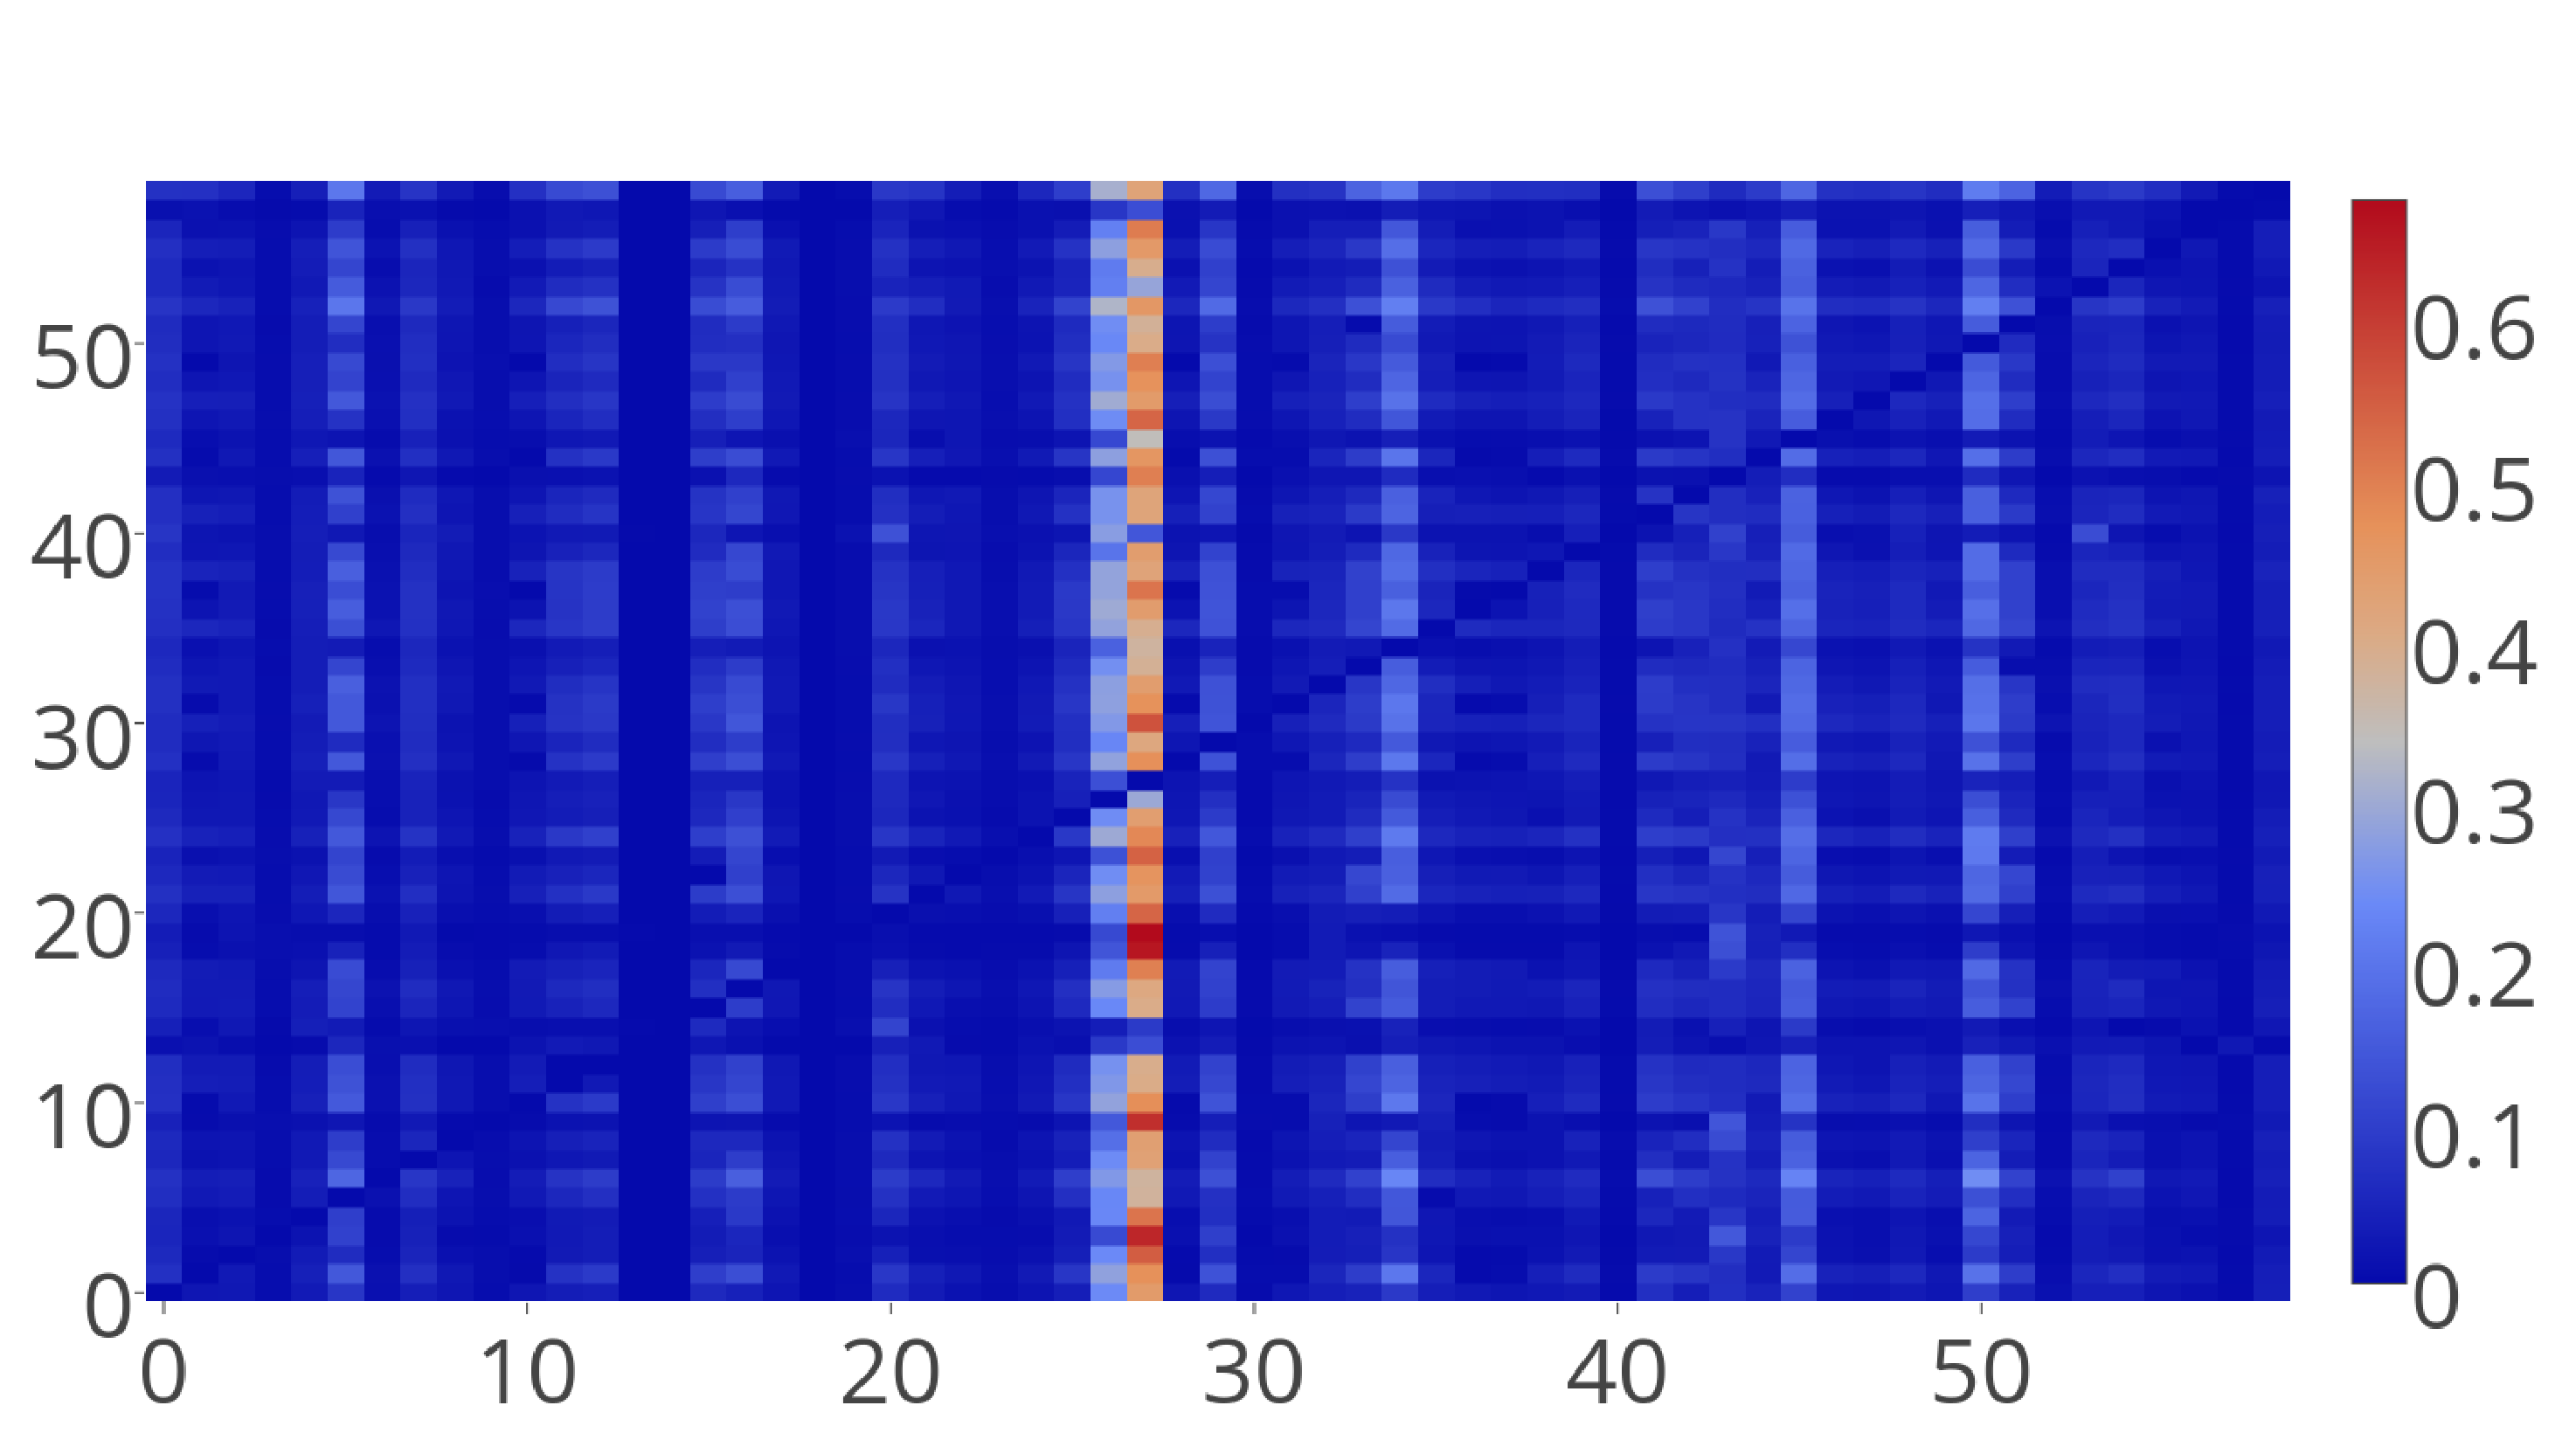
\includegraphics[width=0.24\linewidth]{figure/bernoulli-train}\label{fig:moredata1}} 
\subfloat[]{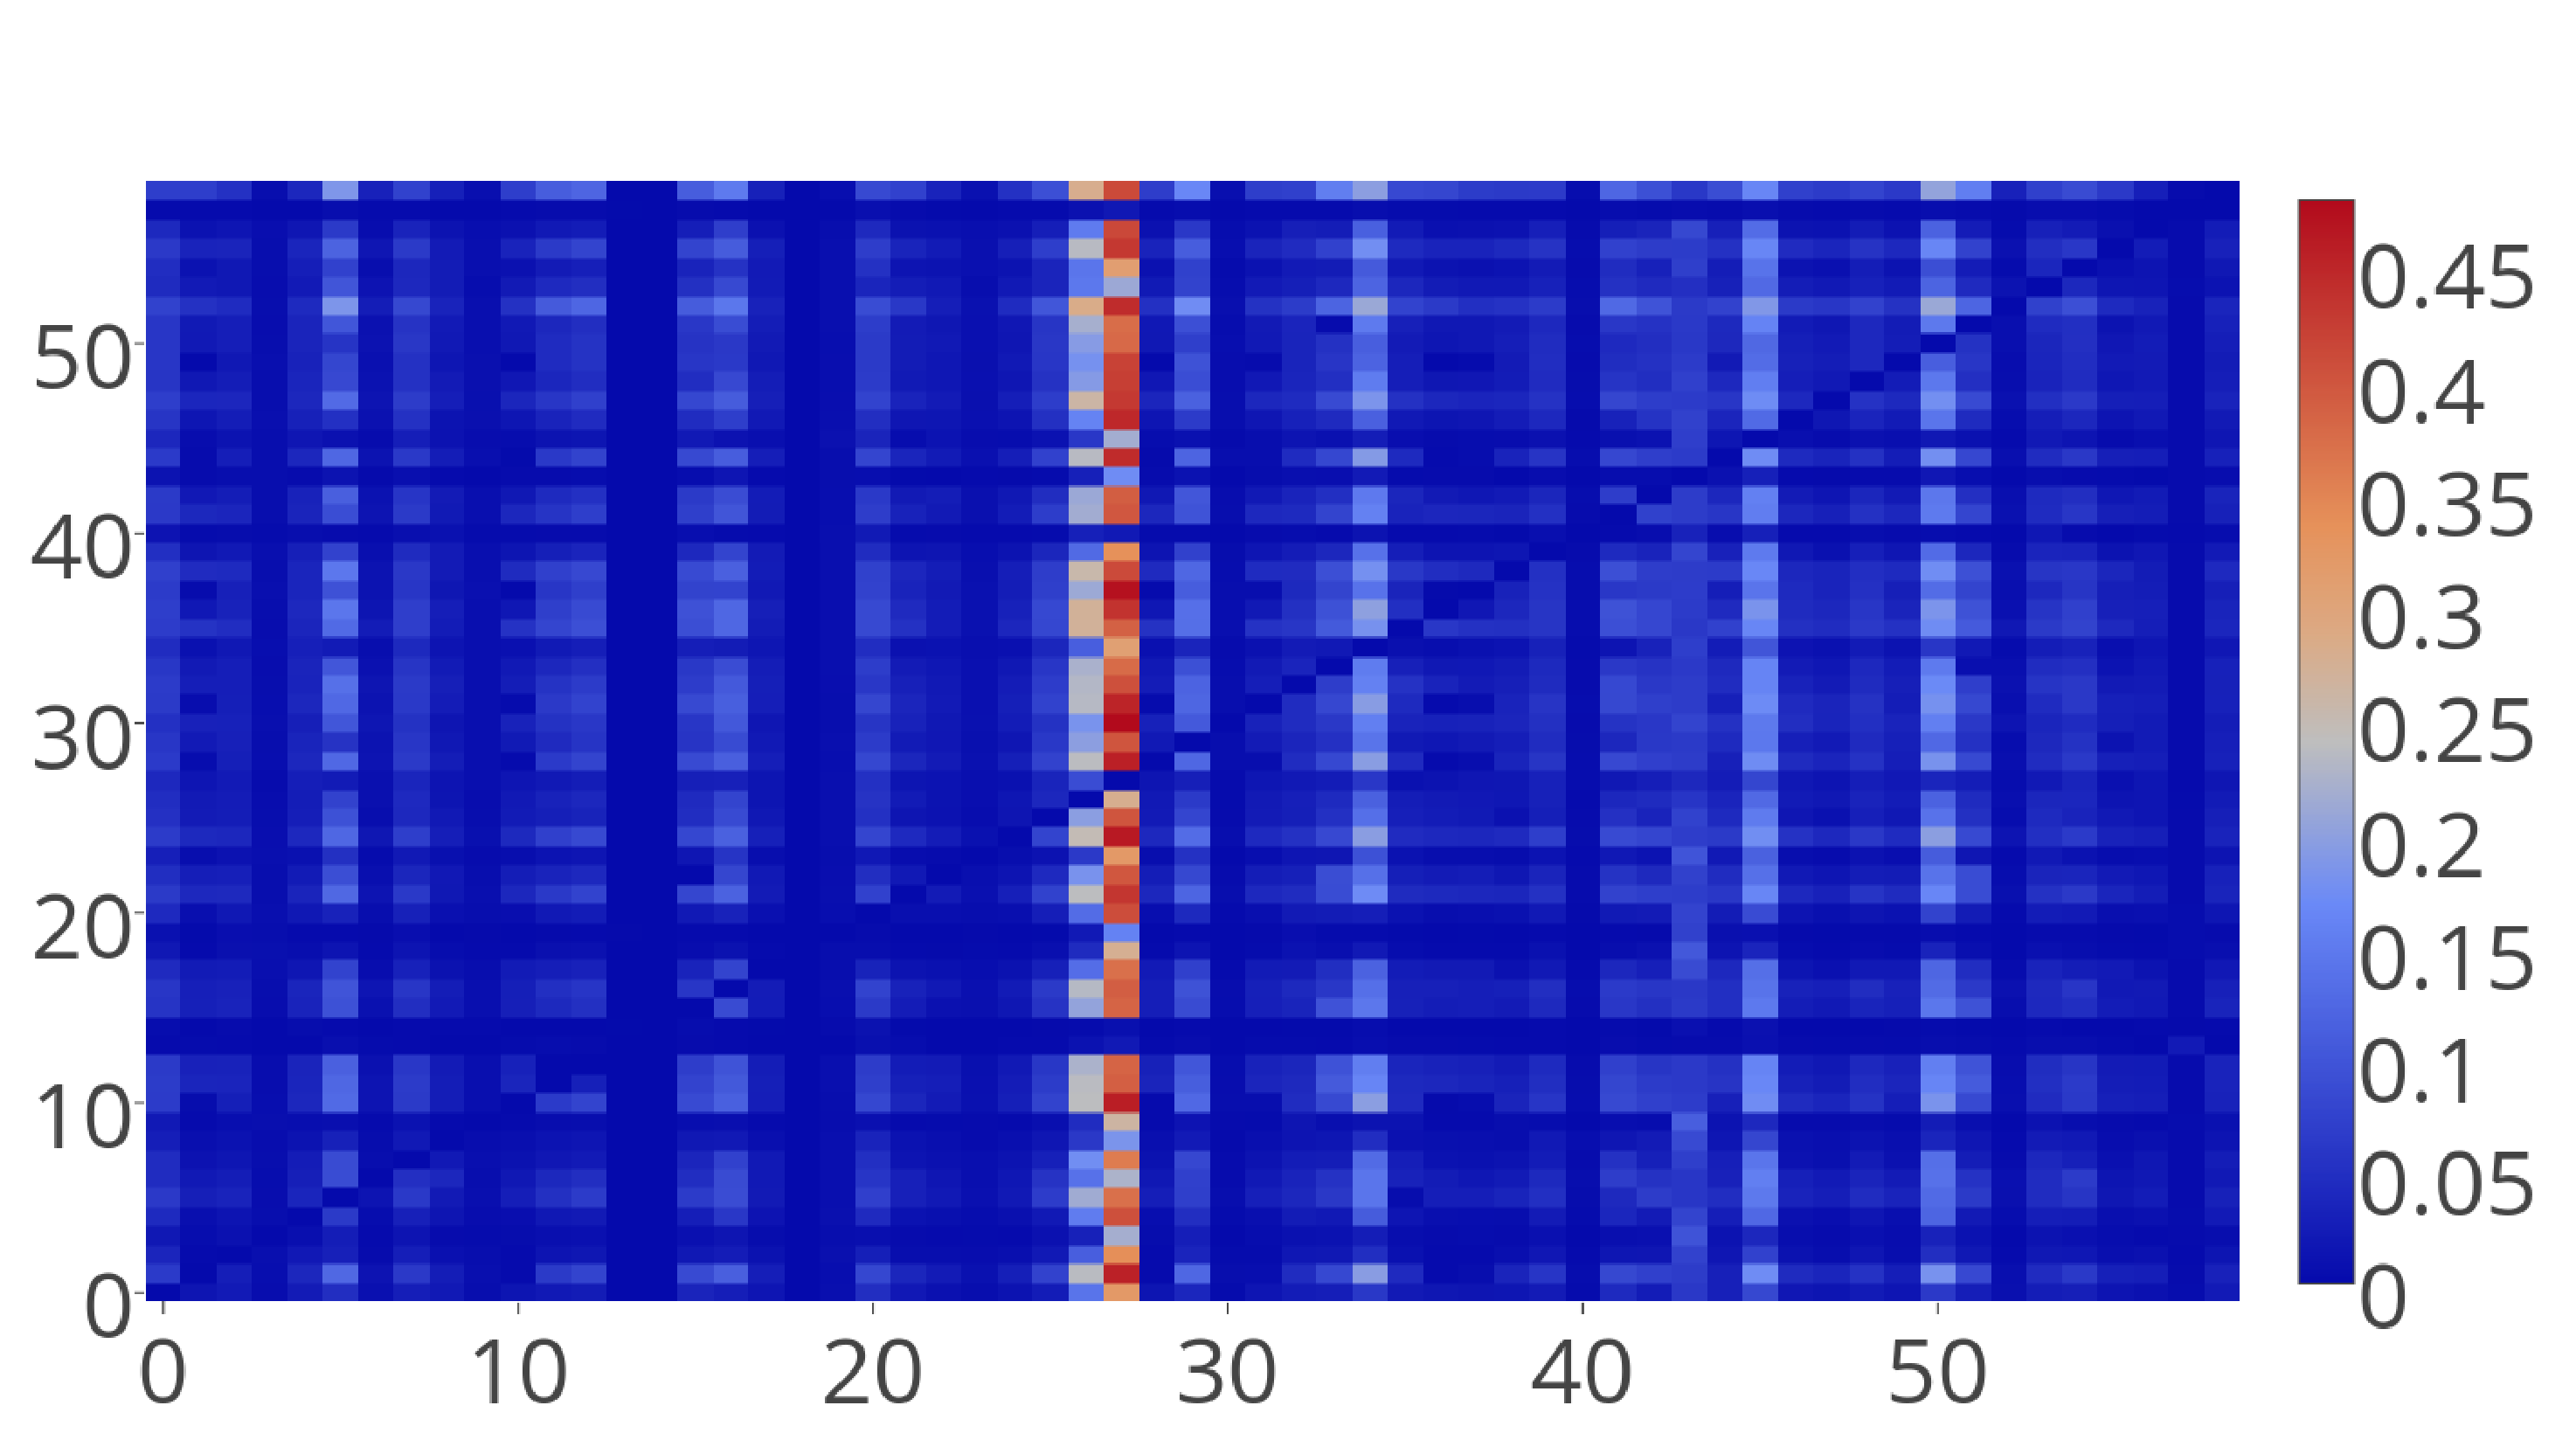
\includegraphics[width=0.24\linewidth]{figure/jaccard-train}\label{fig:moredata2}}
\subfloat[]{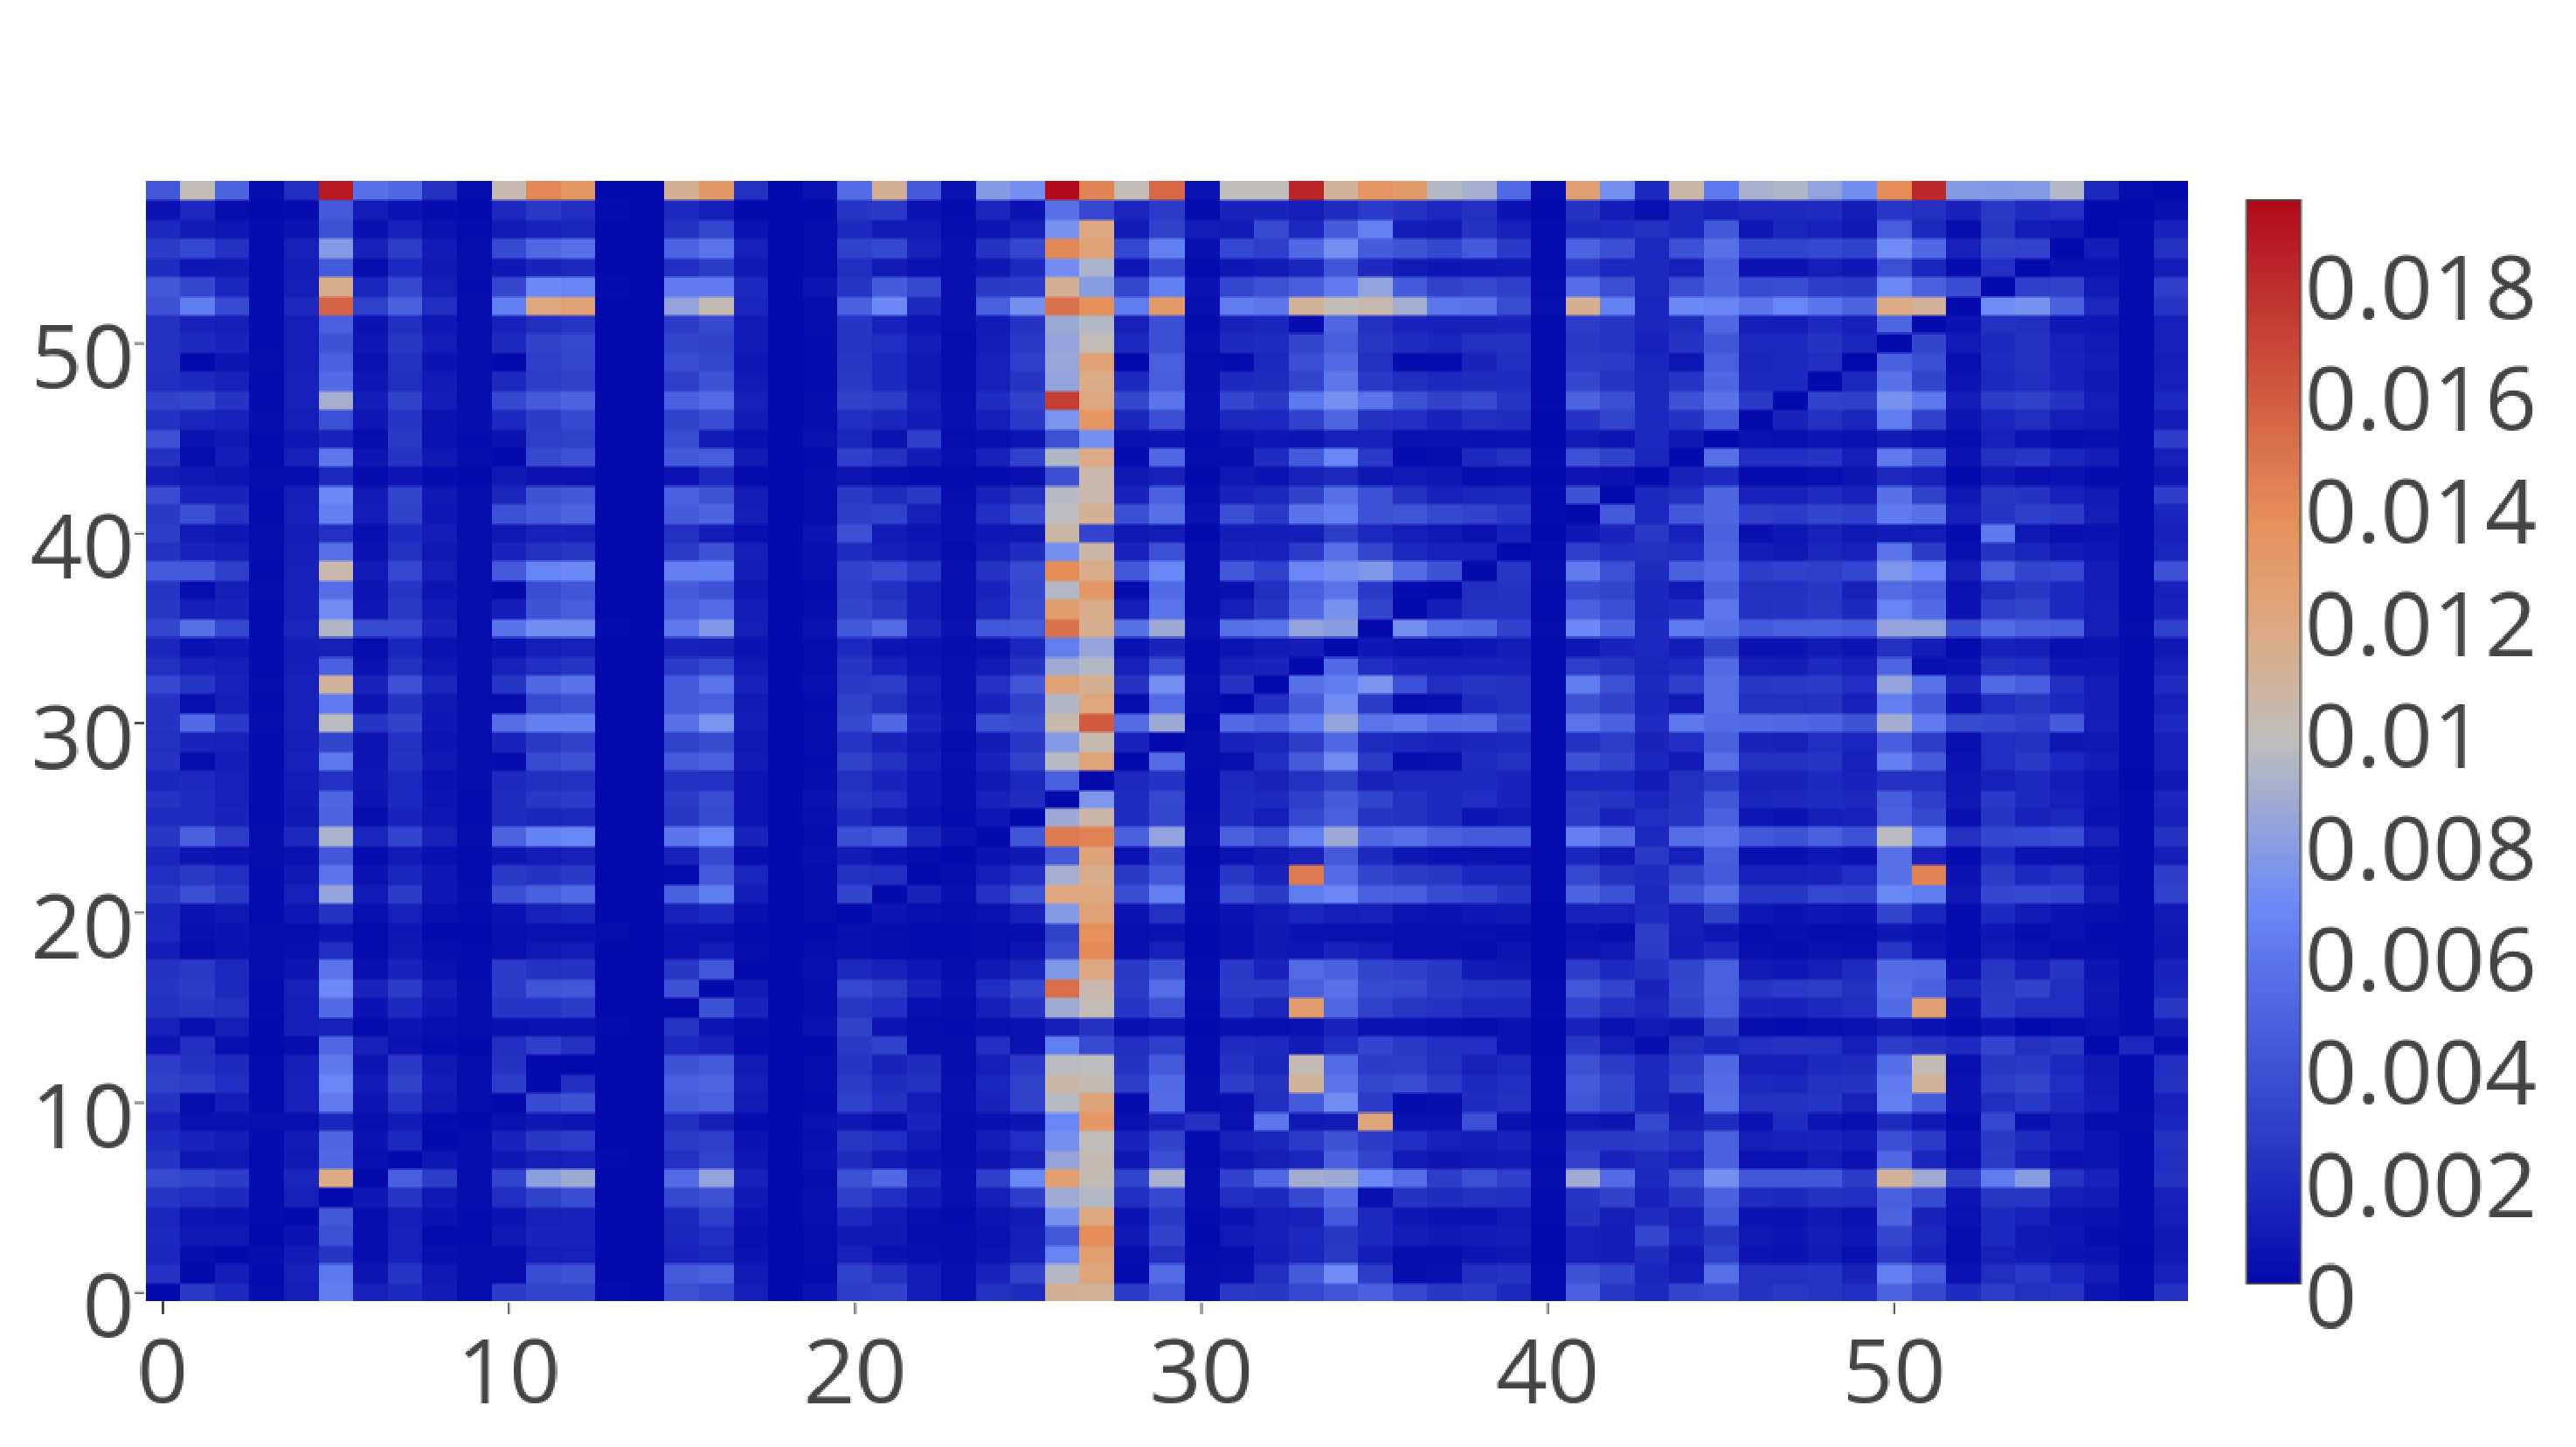
\includegraphics[width=0.24\linewidth]{figure/PC-train}\label{fig:moredata3}} 
\subfloat[]{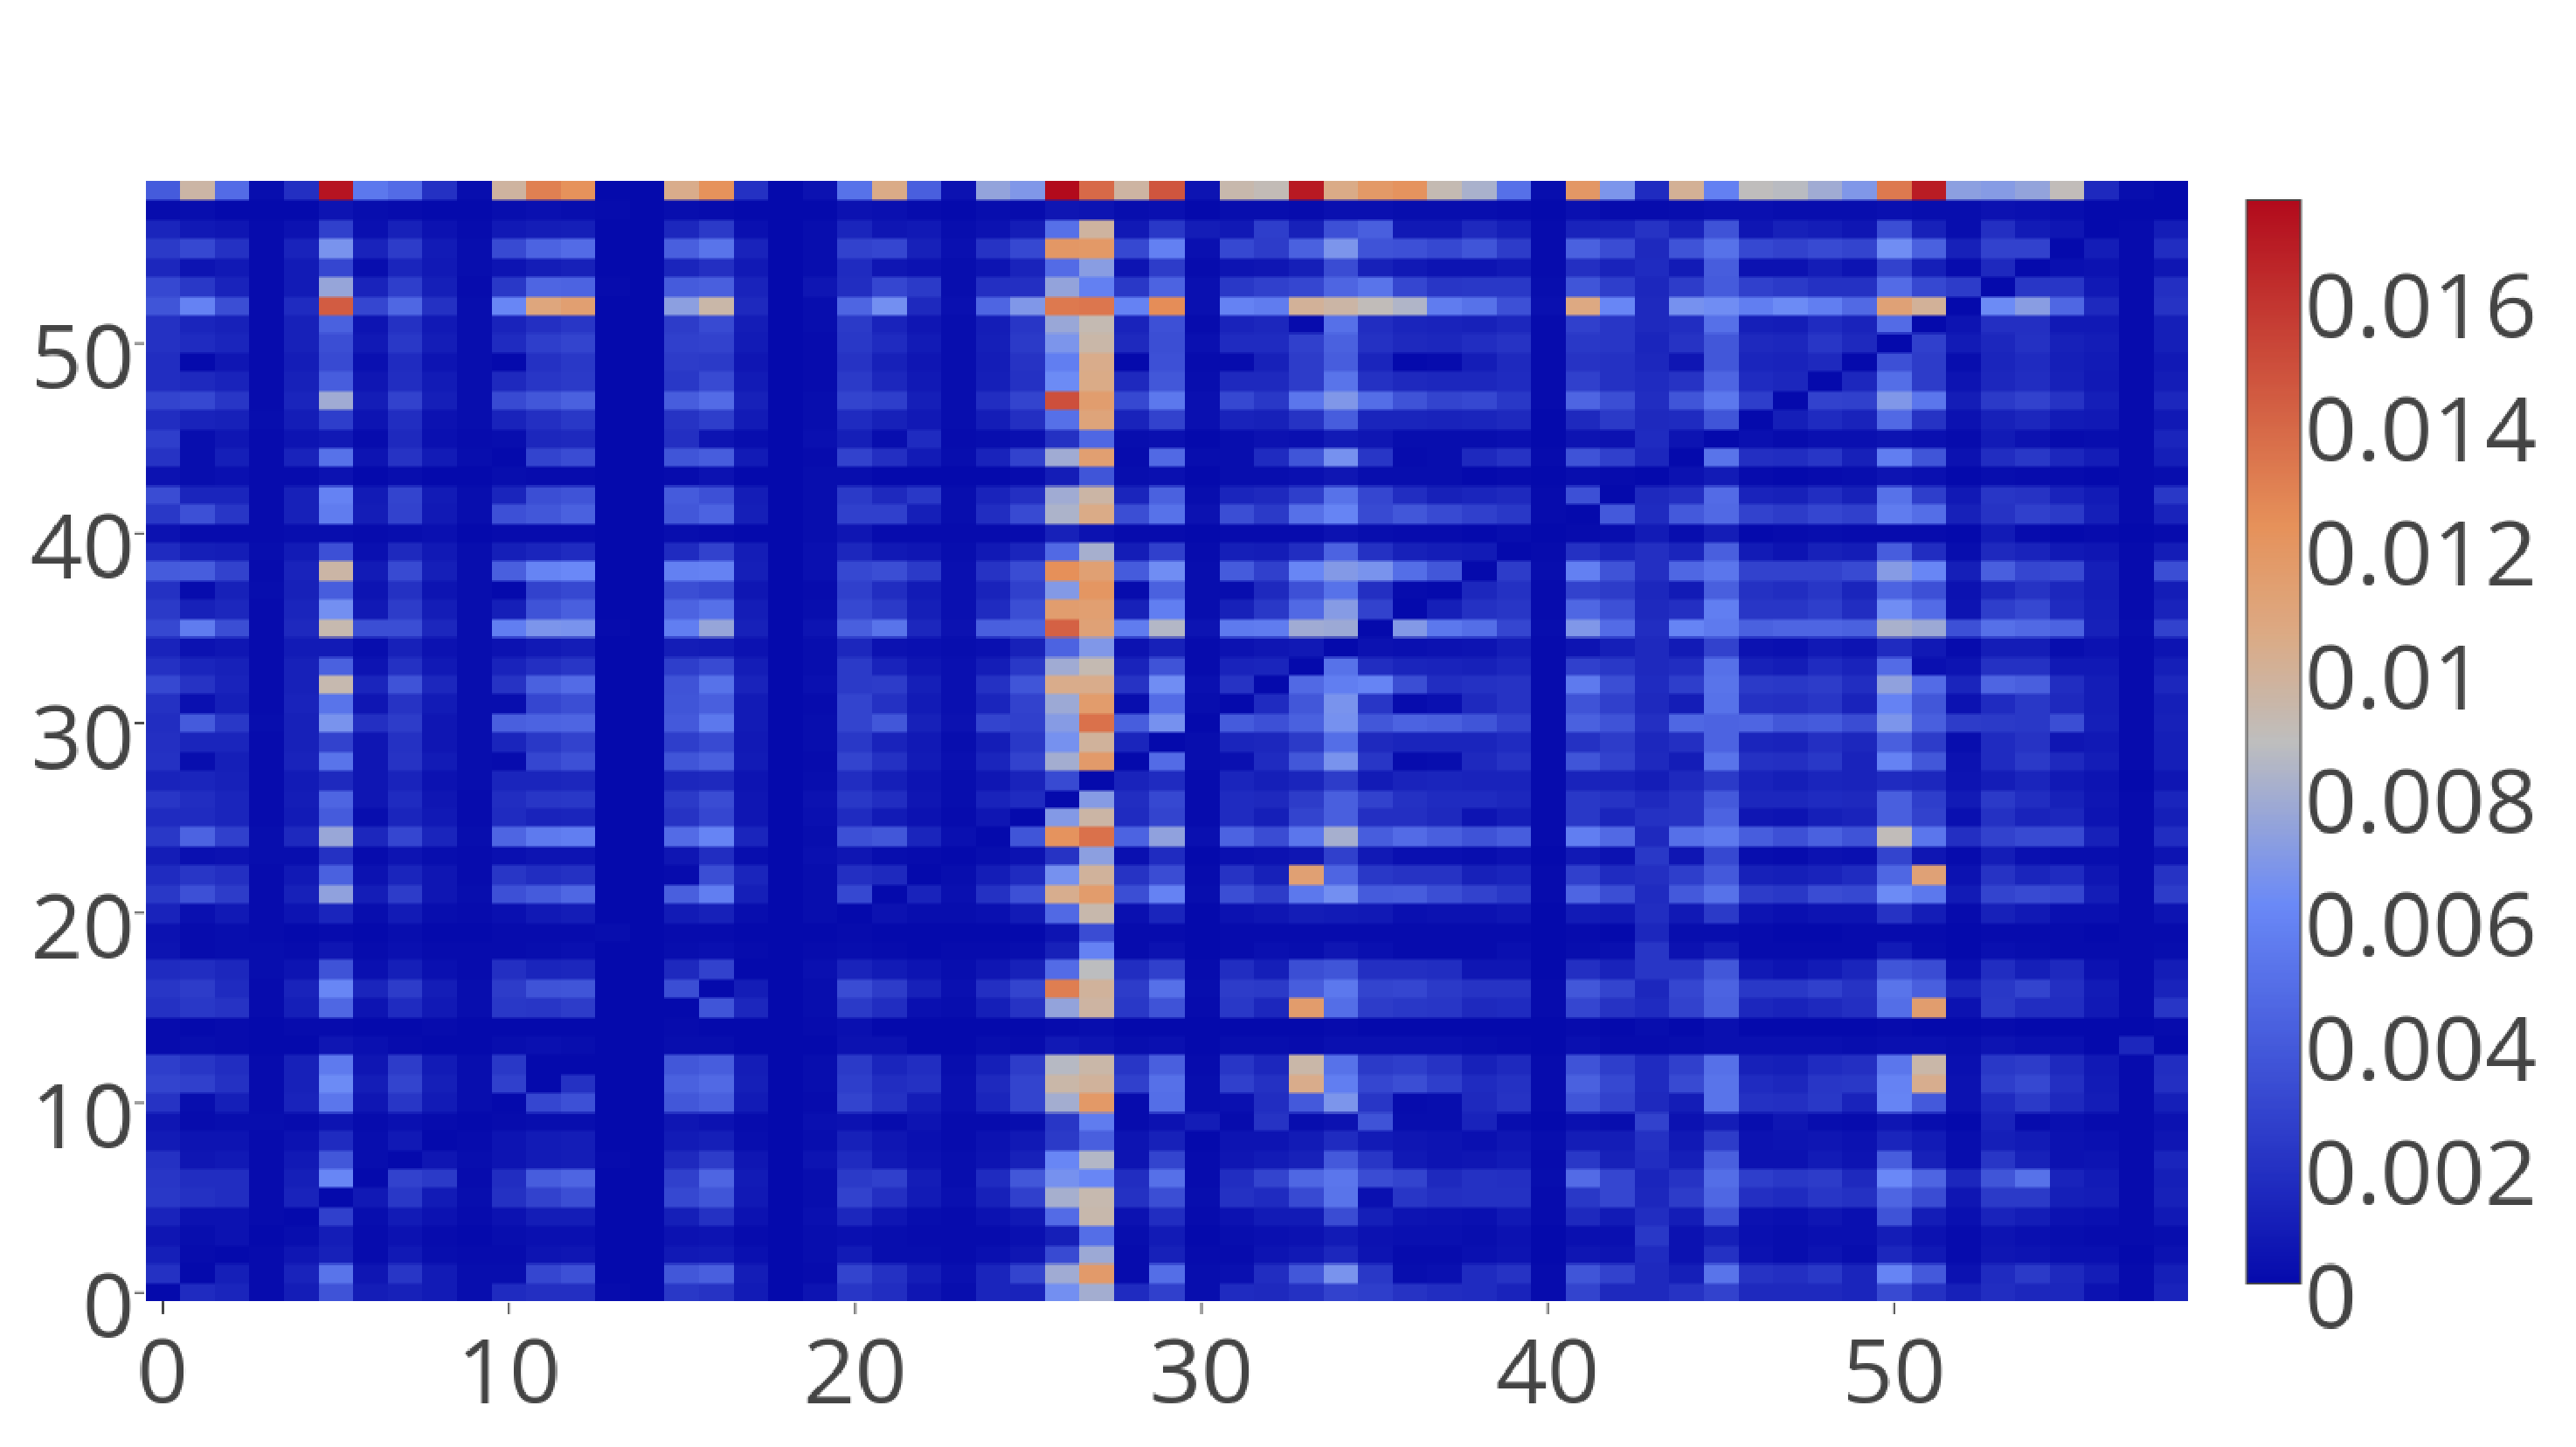
\includegraphics[width=0.24\linewidth]{figure/jaccardPC-train}\label{fig:moredata4}} \\ 
\caption{Potential for 0.5 V bias.} 
\label{fig:EcUND} 
\end{figure*} 


\begin{figure}[t!]
\begin{center}
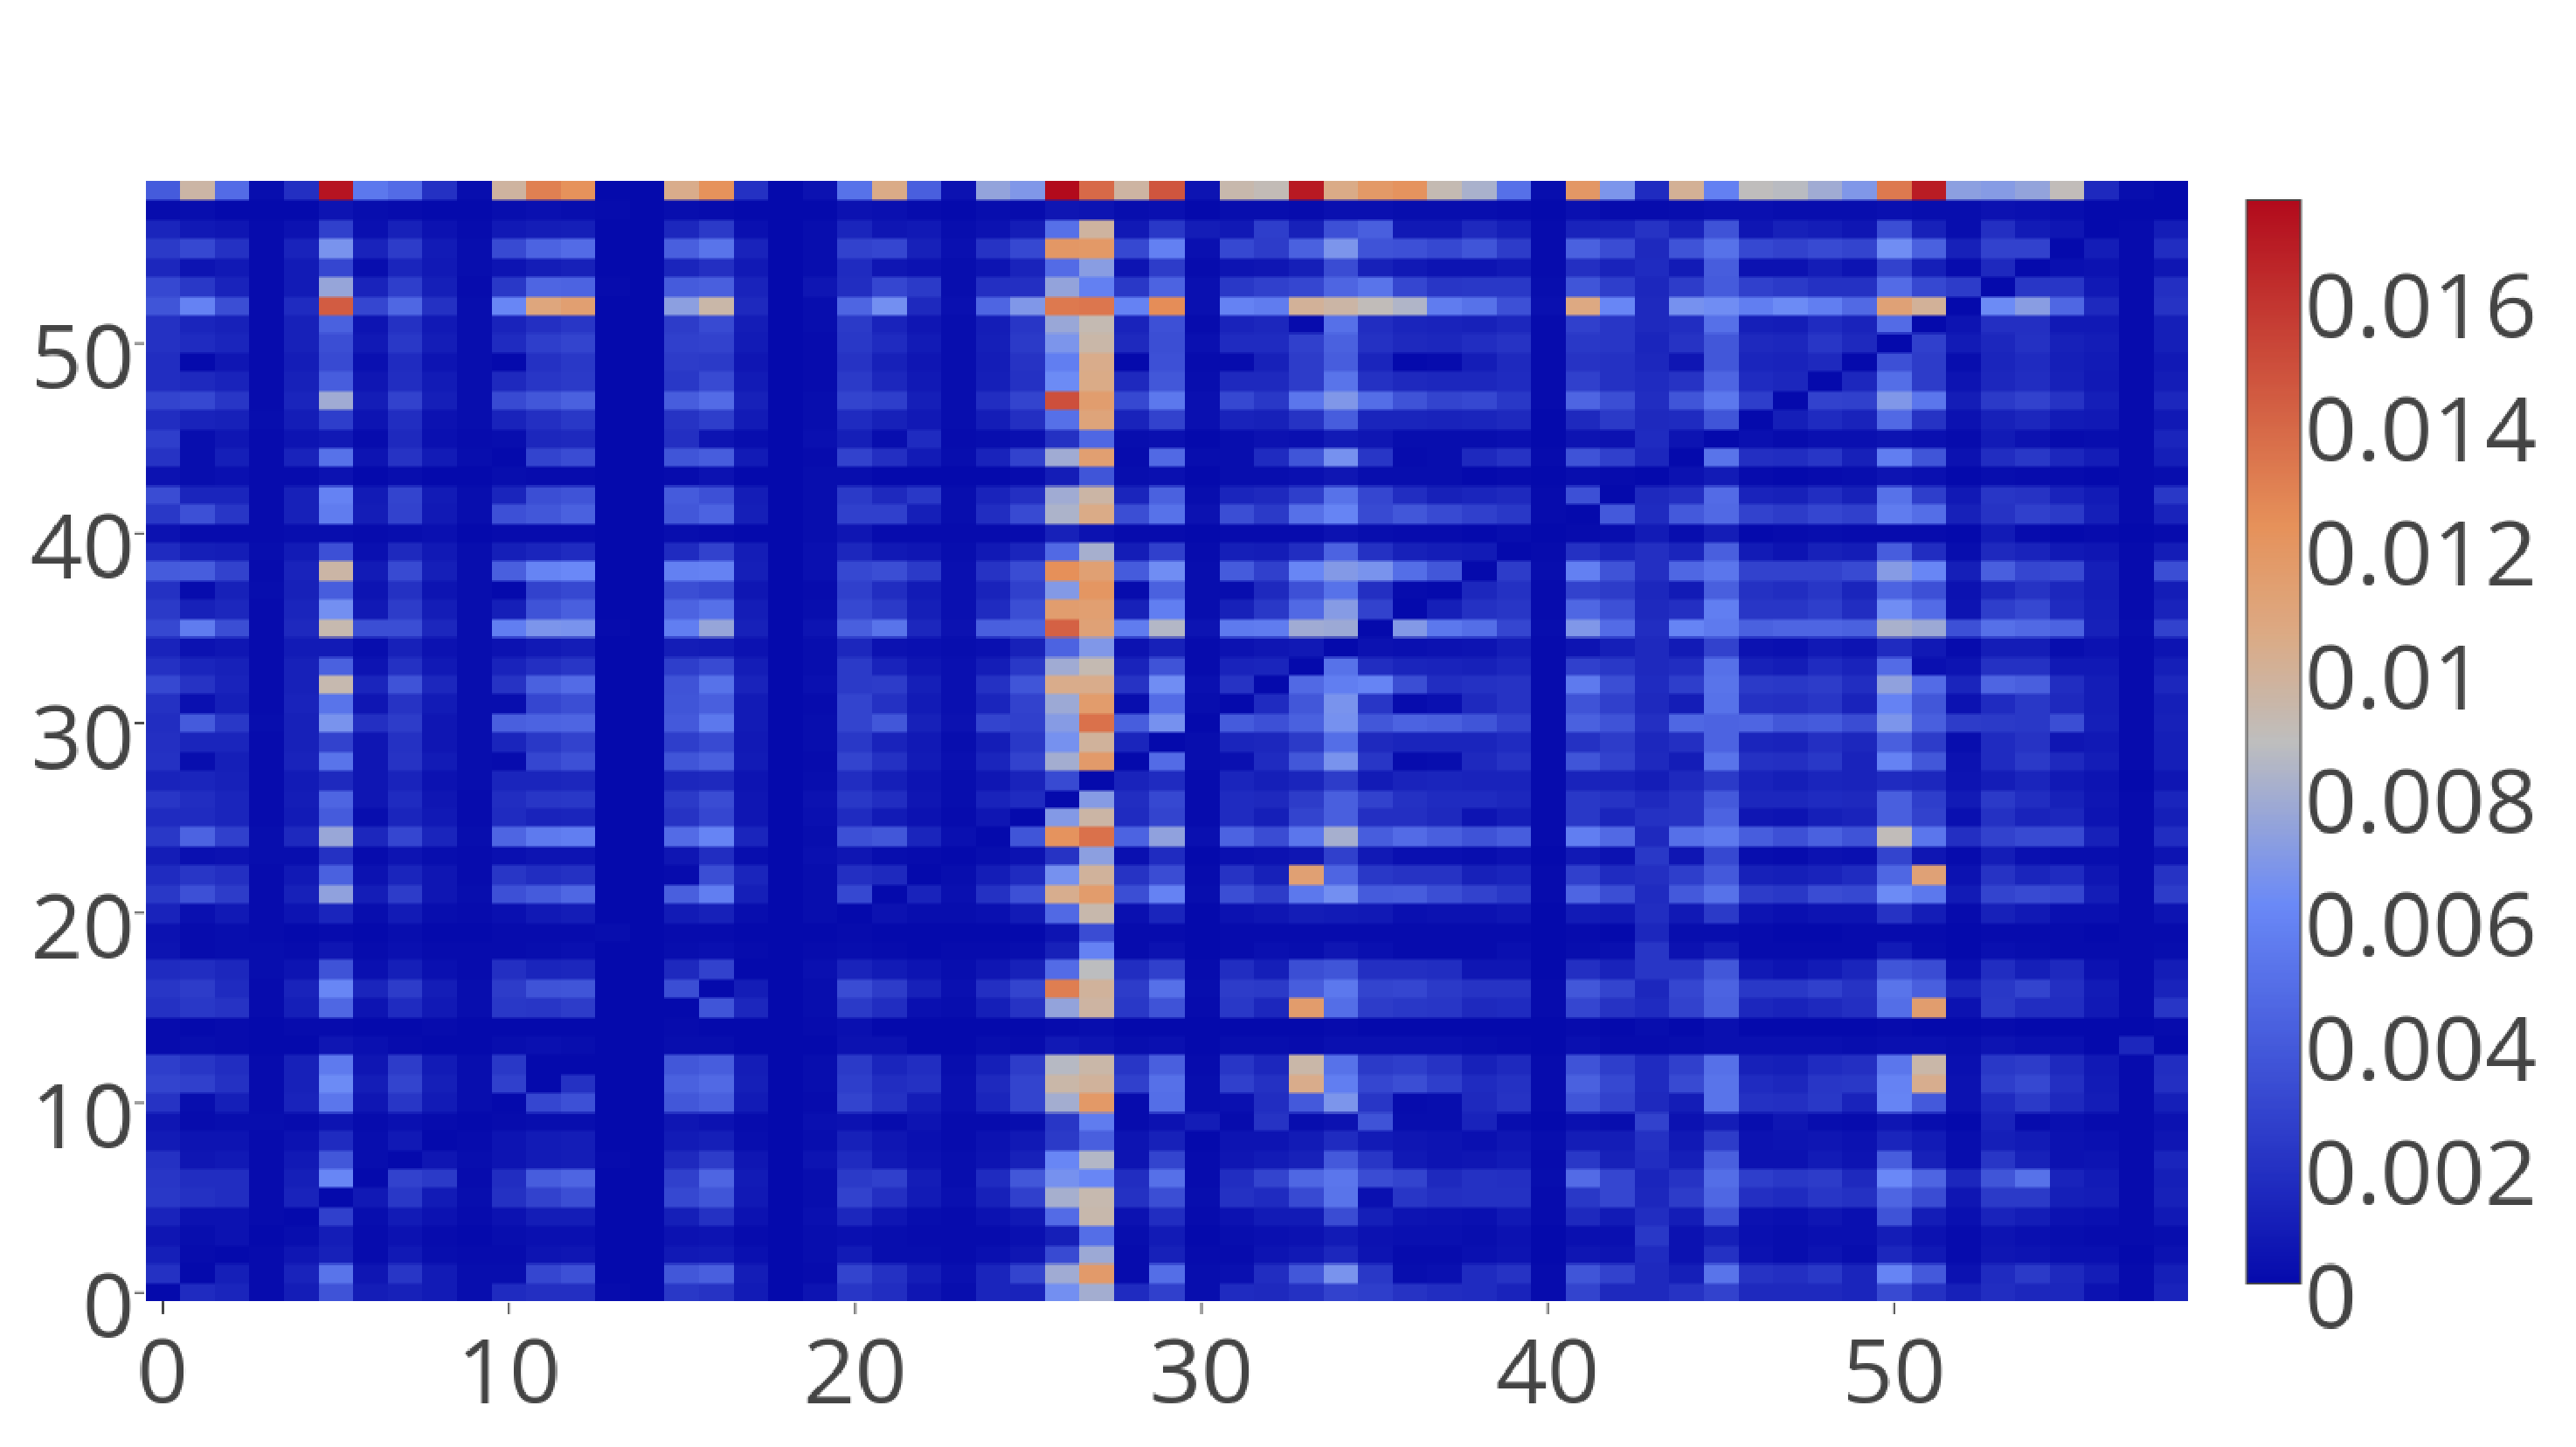
\includegraphics[width=2.5in]{figure/jaccardPC-train}
\mycaption{fig:idreputation}{Test.}
{\footnotesize{(How detection rate changes with the value of source id's reputation. Each reputation is rounded up to nearest 0.05.
Reputation -1 means the source id did not make any submission before. 95\% confidence interval is also drawn 
for each point.)}}
\end{center}
%\vspace{-0.25in}
\end{figure}


\subsection{Influence Probability Analysis}
\label{sec:influenceanalysis}

Using the four static models discussed above, we built an influence graph with anti-virus engines on \vt\ and analyzed 
the influence probability ($p_{u,v}$) between each pair of engines.

\noindent{\underline{\textit{Methodology.}}}
We implement our analysis using several stages of map, filter, and reduce in Spark~\cite{spark}. 
Specifically, we first map submission records according to their corresponding files
and filter out submissions without action propagation. 

\if 0
{\color{red} XXX I don't get the following paragraph. Do we really need this much impl details?}
We then sort submission records for each remaining submitted file chronologically in a map stage.
In the next map stage, we compute four hash tables for each submitted file based on all its submissions.   
There is one one-dimension hash table, containing whether the action to identify the submitted file as malware is taken by each vendor ($|A_{u}|$). 
There are three two-dimension hash tables, 
containing an entry for each pair of vendors $(u,v)$, 
representing whether both $u$ and $v$ take the action ($|A_{u\&v}|$),  
whether the action is propagated from $u$ to $v$ ($|A_{u2v}|$),
and partial credit taken by $u$ if the action is propagated from $u$ to $v$ ($credit_{u,v}(a)$).
After this stage, $|A_{u}|$, $|A_{u\&v}|$, and $|A_{u2v}|$ are either 0 or 1,
and $credit_{u,v}(a)$ is 0 or not larger than 1, since all these values are calculated for one single submitted file. 
In the final stage, 
we reduce these 4 hash tables from different files,
and calculate $p_{u,v}$ for the four static models. 
\fi

We then filter out engines taking fewer than 20000 actions,
since engines taking too few actions cannot produce meaningful results.
There are 59 engines left,
and the average number of actions taken by these engines is around 392K. %190140, which is much larger than 10000.
For confidentiality reasons, we omit vendors' name in the following discussion
and use numbers from 0 to 58 to represent these vendors.

\noindent{\underline{\textit{Analysis results and implications.}}}
For each static model, 
we construct an influence table with calculated influence probability values ($p_{u,v}$), 
with $u$ as row number and $v$ as column number.
We visualize these influence tables with heat maps in Figure~\ref{fig:heat}. 
Each $cell(u, v)$ represents the relative heat color of $p_{u,v}$, 
and red means more influence from $u$ to $v$. 

We also sum all $p_{u,v}$ values in a column in each influence table 
to calculate trustworthiness of engine $v$ using Equation~\ref{eq:trust}. 
Table~\ref{tab:trust} lists the maximum, minimum, and average trustworthiness values of all the engines under four different models.
The results can serve as a quantitative measurement for how trustworthy anti-virus engines are. 

In all the four heat maps, there are two columns with almost all cells in red,
which means that these vendors influenced by all other vendors and are less trustworthy.
On the other hand, quite a few vendors are not influenced by any vendors (blue columns).
This result suggests that most vendors perform predictions on their own and thus can be trusted. 
However, our result should also ring an alarm to online malware detection service users and security experts that 
we cannot treat all engines with the same level of trust 
and the results from some of them should be at least examined more closely if not discarded.

At the same time, there are several rows with many cells in red, especially in the last two heat map, 
which means that there are vendors which influence many vendors,
where there are a set of vendors that do not influence other vendors (blue rows).
Different from the effect of columns which shows the trustworthiness of a vendor by users, 
the effect of rows is related to how vendors view (and trust) each other. 
Certain vendors are highly regarded by many other vendors so that 
their decision results are often referenced by other vendors.

Interestingly, the vendors that are heavily influenced by others are not the ones that influence others, 
suggesting that the vendors with lower trustworthiness by users are also not trusted by other vendors. 

\begin{table}[h!]
\centering
\footnotesize
{
\begin{tabular}{l|l|l|l}
\hline
Model                & Max     & Min & Average \\
\hline                            
%\cline{1-1}
{\bf Bernoulli}                    & 108.78   & 0.04 & 5.40 \\
{\bf Jaccard Index}                & 118.20   & 0.05 & 6.15 \\
{\bf Bernoulli with Partial Credit} & 3545.34  & 1.63 & 138.45 \\
{\bf Jaccard Index with Partial Credit} & 4177.98 & 2.02 & 155.18 \\
\hline
\end{tabular}
}
\caption{Trustworthiness. 
%\footnotesize{
(Maximum, minimum, and average trustworthiness values under four different models.)
%}
}
\label{tab:trust}
\end{table}


Finally, we observe that although the four static models show similar trends of influence relationship 
and the relative rankings of engines in terms of influence are similar,
their absolute influence probability values differ. 
Bernoulli distribution and Jaccard index have influence probability values
that are about 30 to 40 times higher than
Bernoulli and Jaccard index with partial credit. 
%This shows that {\color{red} influence is shared among vendors take actions earlier than others. I have no idea what sentense means. if you cannot explain well, just remove this sentence.}.

{\bf Observation 8:} 
{\em Certain anti-virus vendors are influenced by almost all other vendors in their malware detection decisions and are less trustworthy, 
while quite a few trustworthy vendors have influence on many other vendors.}

\subsection{Influence Probability Prediction}
\label{sec:predict}

The analysis results of vendor influence above are encouraging.
With these results, we take a step further and ask 
{\em if it is possible to predict whether or not an engine's prediction of 
a file submission should be trusted (i.e., not influenced by other engines)?}
We now discuss the prediction model we built to answer this question.

\noindent{\underline{\textit{Methodology.}}}
We first split all the \pe\ submissions we collected into a training set and a testing set based on 
the SHA256 values of the submitted files. 
We place all submissions with SHA256 values starting with a numeric character, 
i.e., from `0' to `9', into training set
and all the rest (starting from 'a' to 'f') into the testing set.
We use Spark to implement both the training and the testing process.
%Similar to our training stage process, 
%we first reduce all submissions based on submitted files,
%next filter out files without action propagation, 
%and then sort submissions chronologically. 


%\noindent{\underline{\textit{Training stage methodology.}}}
During the training stage, we use the training set to build an influence graph and
learn $p_{u,v}$ of each edge in the graph using the four static models discussed in Section~\ref{sec:influenceprob}.
The calculation of $p_{u,v}$ is the same as in Section~\ref{sec:influenceanalysis}.

%\noindent{\underline{\textit{Testing stage methodology.}}}
During the prediction stage, for each submission in the testing set, 
we predict whether or not an engine $v$ will take an action $a$ following other engines 
if it has not taken that action yet. 
%Specifically, we use a tunable threshold $\theta$
%and predict $v$ will follow its neighbors to take the action $a$ in the future
%if $p_v(S_v(a))>\theta$.
Specifically, to test a submission, we first use Equation~\ref{eq:setp} to
calculate $p_v(S_v(a))$, the probability that $v$ will follow its neighbors to take the same action, 
for all engines that have labeled the submitted file only as benign in their history. 
These engines are of interest to us because positive influence, 
the type of influence in this study, only happens 
when an engine changes its prediction decision from benign to malware.

We then compare $p_v(S_v(a))$ with a {\em tunable threshold $\theta$} to predict whether $v$ will label the file as malware (if $p_v(S_v(a))>\theta$) or not.
Next, we compare this prediction with the actual action that $v$ took in the testing set to deduct true positives (TPs) where both our prediction 
and the actual fact label the submission as malware, 
false negatives (FNs) where our prediction labels the submission as benign and the actual labeling is malware. 
Thus, TP means our prediction is the same as the fact 
and both show the engine changes its labeling from benign to malware, an indication that the decision 
of this engine on the submission is in deed affected by other engines.
Similarly, we can obtain false positives (FPs) 
and true negatives (TNs).
%After processing all submissions for a file, 
%we calculate $p_v(S_v(a))$ for all engines  
%that label the file as benign but have not labeled the file as malware.
%We compare $p_v(S_v(a))$ with $\theta$ to count false positives (FPs) and true negatives (TNs).
In the final stage, we calculate the overall TP, TN, FP, and FN rates for all different files.

\begin{figure}[t!]
\begin{center}
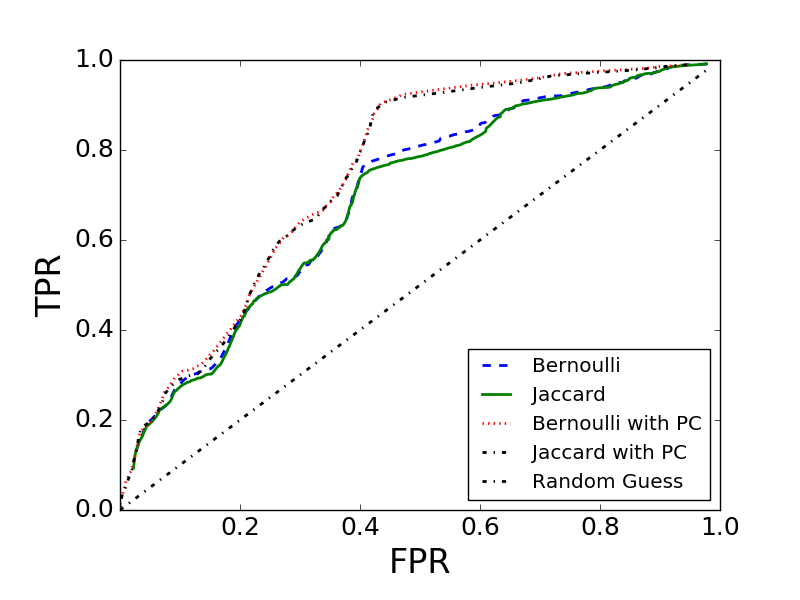
\includegraphics[width=2in]{figure/predict}
\vspace{-0.1in}
\caption{ROC comparisons of Static Models. 
(How true positive rate (TPR) changes with false positive rate (FPR). 
We change probability threshold from 0.1\% to 99.9\% with step 0.1\%. 
We compute TPR and FPR for each probability threshold to draw the curve.)
}
\label{fig:predict}
\end{center}
\vspace{-0.1in}
\end{figure}

\noindent{\underline{\textit{Prediction results.}}}
We change the threshold $\theta$ from 0.1\% to 99.9\% 
and measure the accuracy of the four static models using ROC (Receiver Operating Characteristic) curves,
with true positive rate ($TPR = TP/(TP+FN)$) as X-axis
and false positive rate ($FPR = FP/(FP + FN)$) as Y-axis. 
Figure~\ref{fig:predict} plots the ROC curves for the four static models.
A larger area under the ROC curve means higher accuracy.
We compare our prediction models with random guess, 
which is represented by the diagonal line between (0,0) to (1,1) in the figure. 

We find that all models are more accurate than random guess
and using partial credits improves the accuracy of both Bernoulli and Jaccard index.
This result is encouraging;
even with a simple prediction model like ours, we can already obtain satisfactory prediction accuracy of whether an engine's decision has been influenced by others.

{\bf Observation 9:} 
{\em Our influence prediction model can accurately predict whether or not an anti-virus engine's labeling of a submission should be trusted. }

\subsection{Discussion}
%Our scientific analysis on vendor influence in this section confirms our XXX
Our findings in this section shed light on how vendors can influence each other and rings an alert towards using detection rate as the only measurement of the likelihood of a file being malware.
Our study results can serve as a quantitative measurement for vendors' influence in malware detection community. 
Previously, when combining results from different vendors, 
security experts simply treat each vendor equally and use the percentage of 
vendors labeling a file as malware as likelihood of the file to be a malware. 
Our model can provide a weight to each vendor 
when combining results from different vendors.  
Anti-virus vendors can also use our prediction model to detect possible false negatives in their products.

\if 0
{\color{red} Do we really need this (the following two paragraphs)? this sounds very defensive}
%\if 0
There are also time models proposed by~\citet{Influence}.
When analyzing Flickr data, time models leverage accurate action time to provide better prediction performance. 
However, we do not use time models, 
because time information we access is when a submission is conducted, 
or when an engine analyzes a submission, 
is not when an engine changes its detection label for a file.
The time information we have can only provide a relative order about when each vendor identifies a file as malware.  

%\underline{Limitation.}
Our data collection ends on September 6th, 2016. 
We could count extra FPs, where we predict engines will label files as malware, engines have not, but will do in the future, 
and TNs, where we predict engine will not label, engines have not, but will in the future. 
Monitoring \vt for a longer time will make the evaluation of our prediction models more precise. 

%\underline{How to use?}
\fi


%\section{Malware Classification}
\label{sec:ssdeep}

Machine learning systems are just as good
as the data they consumed---One potential 
use case of the massive amount of data 
available on VirusTotal is to build 
machine learning models for applications
such as malware classifications and
clustering. In this section, we study
the question that {\em Is the data
provided by VirusTotal enough to support
classifications and clusterings tasks?}

Our study reveals both positive and
negative answers to this question---For
some classification tasks, we are able
to build an automatic classifier whose
accuracy is higher than 80\% by just
using the static signature provided by VirusTotal
and we expect the quality to keep increasing
given more data; on the other hand,
we identify some classification tasks
whose accuracy hardly beat random guesses.
We also identify a simple metrics
to predict whether a given task belongs
the high-quality category or the low-quality
category. We hope our study shed lights
on future design of signatures for malware
detection.

%Malware detectors mainly rely on signatures manually extracted by security researchers. 
%ssdeep only takes static binary executable as inputs. 
%If we can build malware detector based on ssdeep similarity, 
%We can reduce or even eliminate manual efforts in malware detection. 


\subsection{Data Collection}

\begin{table*}
  \centering
  \scriptsize
  {
  \begin{tabular}{clccc}
    \toprule
{\bf Index} & {\bf Microsoft Tag} & {\bf \# of Malwares} & {\bf \% of Tailing}  & {\bf \% of Distinct}\\
\midrule                                                                                                                                                                                                                                           
1  &  SoftwareBundler:Win32/Penzievs 	& 49380	     & 3.51\%  & 99.98\%\\
2  &  Adware:Win32/Hotbar               & 132161   & 1.88\%  & 99.98\%\\
3  &  TrojanDropper:Win32/Lamechi!rfn	& 39205	     & 0.01\%  & 6.13\%\\
4  &  Virus:Win32/Nabucur.D	            & 1190132  & 99.95\% & 100.00\%\\
5  &  Virus:Win32/Virut.BO	            & 84600	   & 21.84\% & 99.95\% \\
6  &  Worm:Win32/Mydoom.L@mm	        & 76259	     & 0\%     & 99.44\%\\
7  &  Virus:Win32/Ramnit.I              & 412052   & 3.07\%  & 96.76\%\\
8  &  Trojan:Win32/Dorv.A               & 54324    & 2.80\%  & 80.53\%\\
9  &  Trojan:Win32/Dynamer!ac           & 145402   & 65.17\% & 99.20\%\\
10 &  Virus:Win32/Ramnit.A              & 181524   & 26.79\% & 99.82\%\\   

\bottomrule
   \end{tabular}
   }
   \mycaption{tab:benchmark}{Benchmark Information.}
{\footnotesize{(Information for malwares used in our clustering and classification experiments. \# of Malwares: \# of distinct malwares we collected in each sampled malware group from 05/07/2016 to 09/06/2016. \% of Tailing: \% of tailing examples in each group. \% of Distinct: number of distinct ssdeep hash strings divided by group size.)}}
  %\nocaptionrule
  %\mycaption{tab:benchmark}{Malware Data Set.}
  %\footnotesize{(Information for malwares used in our clustering and classification experiments. \# of Malwares: \# of distinct malwares we collected in each sampled malware group from 05/07/2016 to 09/06/2016. \% of Tailing: \% of tailing examples for each group in the sampled 10000 malwares.)}
 %}
\end{table*}




Our study uses features based on ssdeep~\cite{ssdeep}, a program to compute fuzzy hashes. 
Similarity between calculated hash strings can serve as an estimation for similarity between the two original files. 
ssdeep hash strings are also provided for each submitted file with other metadata fields by \vt. 

We focus on classifying each malware into
different malware families. Because Microsoft 
has a good reputation in detecting PE malwares~\cite{SongAPsys2016}, we create training
data using its assignment. For each detected malware, Microsoft assigns it a tag, which contains type, platform, family, and variant information~\cite{microsoft}. 
We divide PE malwares detected by Microsoft engine into different groups, and malwares in the same group share the same Microsoft malware tag. 
We sample 10 groups, each of which with more than 10000 malwares.  
Microsoft tag and number of malwares in each sampled group we collected from \vt{} are shown in Table~\ref{tab:benchmark}. 
For each group, we sample 10000 malwares, and use these malwares in our following experiments. 


\subsection{Classification Accuracy}

We build an classifier as follows. \ce{XXXX LINHAI, ADD IN THE PROTOCOL.}

Table~\ref{tab:results} shows the classification
result and Figure~\ref{fig:moredata} shows
the relationship between the amount of
training data and the accuracy of classifiers. 
We see that for five out of ten 
malware families, we achieve an accuracy
higher than 80\%. Moreover, as indicated
by Figure~\ref{fig:moredata}, when more
training data are available for these
families, we expect the accuracy to be even
higher. On the other hand, for
families such as ``Virus:Win32/Nabucur.D'',
the classification accuracy are significant
lower. We get an accuracy of 59\% when
\ce{the accuracy of random guesses would be 50\%. LINHAI IS THIS RIGHT?}
\ce{LINHAI, ADD ONE SENTENCE ABOUT THE REASON.}

\paragraph*{Discussion: Tailing Malwares}

We identify one metrics to predict whether
a classification task falls into the
high-accuracy category or low-accuracy
category. The intuition is that the probability
that a given sample has similar samples in
the training set is a proxy of the upper bound
of accuracy that we can expect. Therefore,
we compute the percentage of tailing malwares in each group--We call malwares, which have 0 similarity with all the other samples in the same group, as tailing malwares. 
The percentage of tailing malwares for each sampled group is also shown in Table~\ref{tab:benchmark}. 

\ce{LINHAI, ADD IN THAT \#TRAILING-VS.ACCURACY FIGURE AND ARGUE ABOUT CORRELATION HERE.}

\paragraph*{Discussion: Challenge of Applying Nystrom Methods for Kernel Machines}

\begin{table*}
\centering
\footnotesize
{
\begin{tabular}{cccccccccccc}
 \toprule
  & \multicolumn{9}{c}{Clustering} &\multicolumn{2}{c}{Classification}\\
\cline{1-1}
\cline{2-10}
\cline{11-12}
 \bf{Index}             & {\bf 0.1}  & {\bf 0.2} & {\bf 0.3} & {\bf 0.4} & {\bf 0.5}  & {\bf 0.6} & {\bf 0.7} & {\bf 0.8} & {\bf 0.9} & {\bf Best k} & {\bf Precision} \\
              \midrule  
          1   & 2483       & 575       &  503      &   456     & 443        & 381       & 356       & 356       & 356       &     1        & 81.27\%  \\
          2   & 4192       & 762       &  635      &   588     & 580        & 534       & 526       & 526       & 526       &     1        & 82\%     \\
          3   &  5         & 4         &  3        &    2      & 2          & 2         & 2         & 2         & 2         &     1        & 82.55\%  \\
          4   & 10000      & 9999      & 9998      & 9997      & 9997       & 9997      & 9997      & 9997      & 9997      &     2        & 59.81\%  \\
          5   & 8688       & 7727      & 6630      & 5462      & 4699       & 3690      & 3103      & 3028      & 3028      &     1        & 76.23\%   \\
          6   & 5807       & 3915      & 1590      & 373       & 18         & 1         & 1         & 1         & 1         &     3        & 81.79\%   \\
          7   & 5429       & 3651      & 2703      & 1615      & 726        & 400       & 369       & 362       & 362       &     1        & 81.79\%   \\
          8   & 2721       & 1400      & 871       & 642       & 549        & 420       & 399       & 396       & 396       &     1        & 82.26\%    \\
          9   & 8500       & 8199      & 8012      & 7808      & 7597       & 7327      & 7171      & 7150      & 7150      &     1        & 64.41\%    \\
          10  & 8075       & 7241      & 6343      & 5193      & 4382       & 3800      & 3506      & 3480      & 3480      &     1        & 74.06\%    \\

\bottomrule
\end{tabular}
}
 \mycaption{tab:results}{Clustering and Classification Results.}
{\footnotesize{(Numbers of resulting clusters under distance threshold from 0.1 to 0.9 are shown in \bf{Clustering} column. K with best precision during cross validation and precision of knn with best k are shown in \bf{Classification} column.)}}
%\caption{Clustering and Classification Results. \footnotesize{(Numbers of resulting clusters under distance threshold from 0.1 to 0.9 are shown in \bf{Clustering} column.
%K with best precision during cross validation and precision of knn with best k are shown in \bf{Classification} column.)}
%}
\end{table*}

Our previous experiment uses k-means classifier.
In this section, we discuss the potential of using
more sophisticated classifiers such as
support vector machines. One challenge
of applying kernel machines is to
approximate the kernel matrix whose
size is quadratic to the number of samples
in the training set. Nystrom Methods~\cite{clustering-purpose} are popular ways to
approximate a kernel matrix with clusters.

To understand the potential of applying Nystrom Methods, we run hierarchical clustering~\cite{hcluster} on our data.
Hierarchical clustering starts with each instance as a cluster, 
and then it iteratively merge two clusters with minimum distance 
until distance threshold or cluster number threshold is reached. 
We use distance as threshold. 
Given two malwares, 
we use 1 to minus their ssdeep similarity to calculate distance between the two malwares. 
We calculate single linkage distance as distance between two clusters. 
Single linkage
distance~\cite{single-link} when we need to compute distance between two clusters. 

We change distance threshold from 0.1 to 0.9, 
and count resulting clusters under each experiment. 
Experimental results are shown in Table~\ref{tab:results}. 
As we increase distance threshold, the number of resulting clusters decreases for each sampled group. 
The number of resulting clusters is always bounded by the number of tailing in each group. 
If we want to change a ssdeep hash string to a feature vector, 
based on distance of the string to the center of all clusters in training set, 
the size of the resulting feature vector would have a very large variance across different malware groups. 
\ce{This illustrates a challenge of directly applying
classic Nystrom method, however, we believe
it is possible to develop new approaches to
accommodate this observation in the future.}

\begin{figure*}
\centering
\subfloat[Group 1]{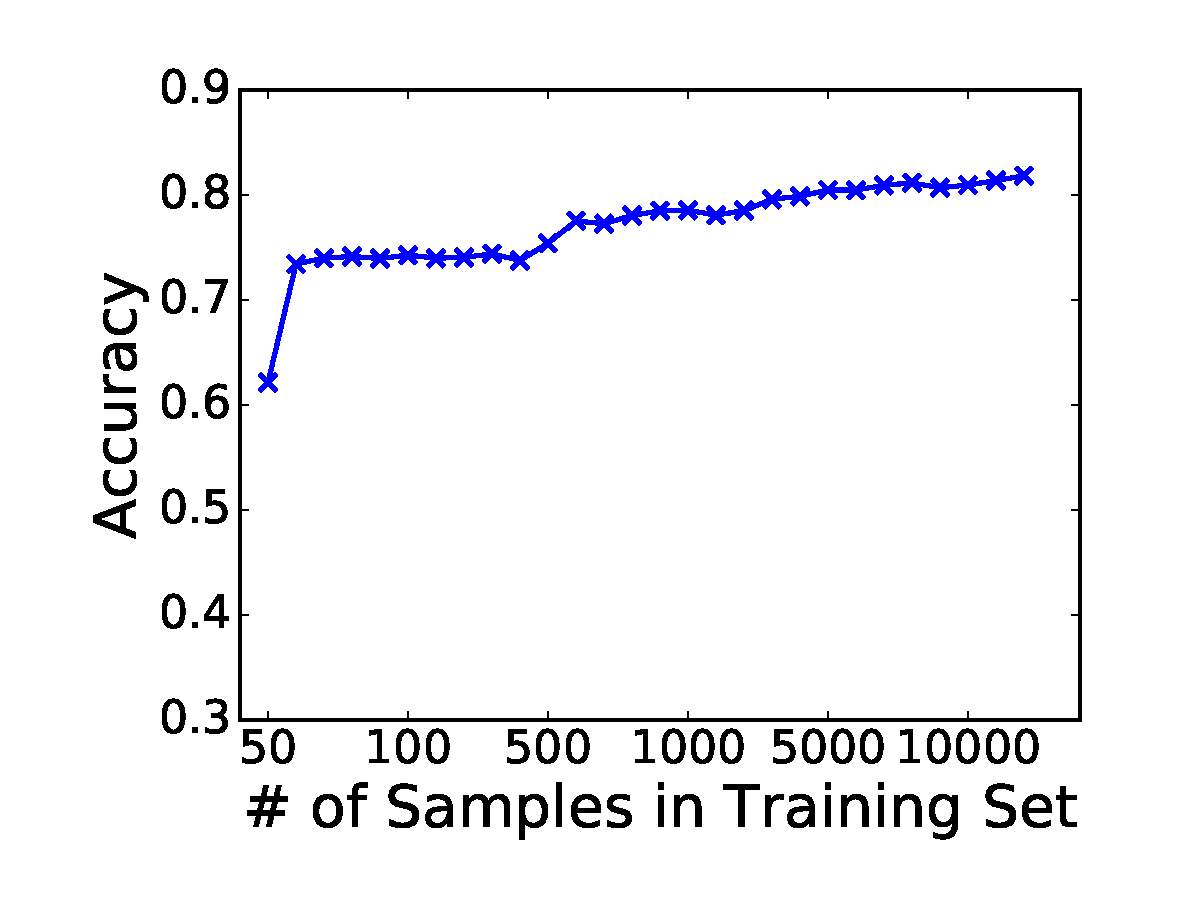
\includegraphics[width=0.16\linewidth]{figure/svm/0}\label{fig:moredata1}} 
\subfloat[Group 2]{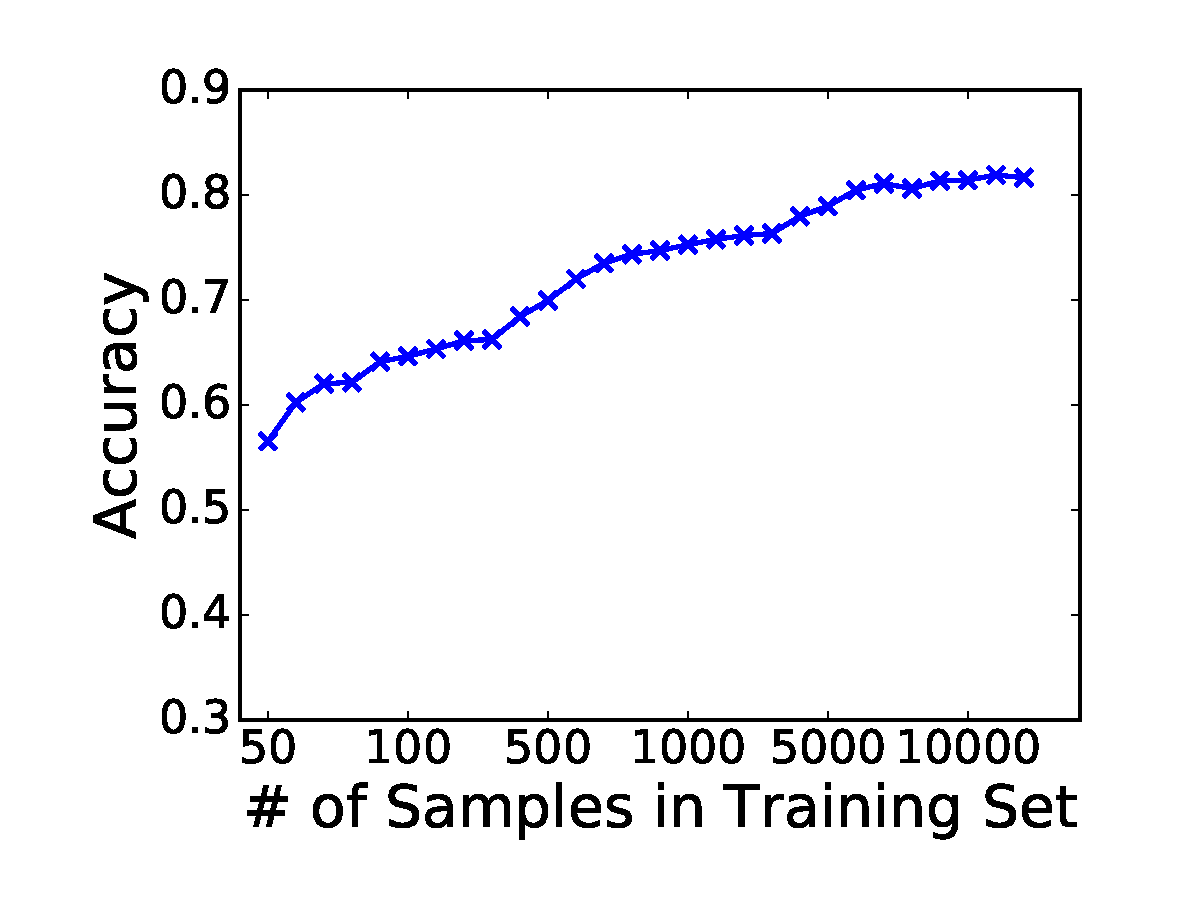
\includegraphics[width=0.16\linewidth]{figure/svm/1}\label{fig:moredata2}}
\subfloat[Group 3]{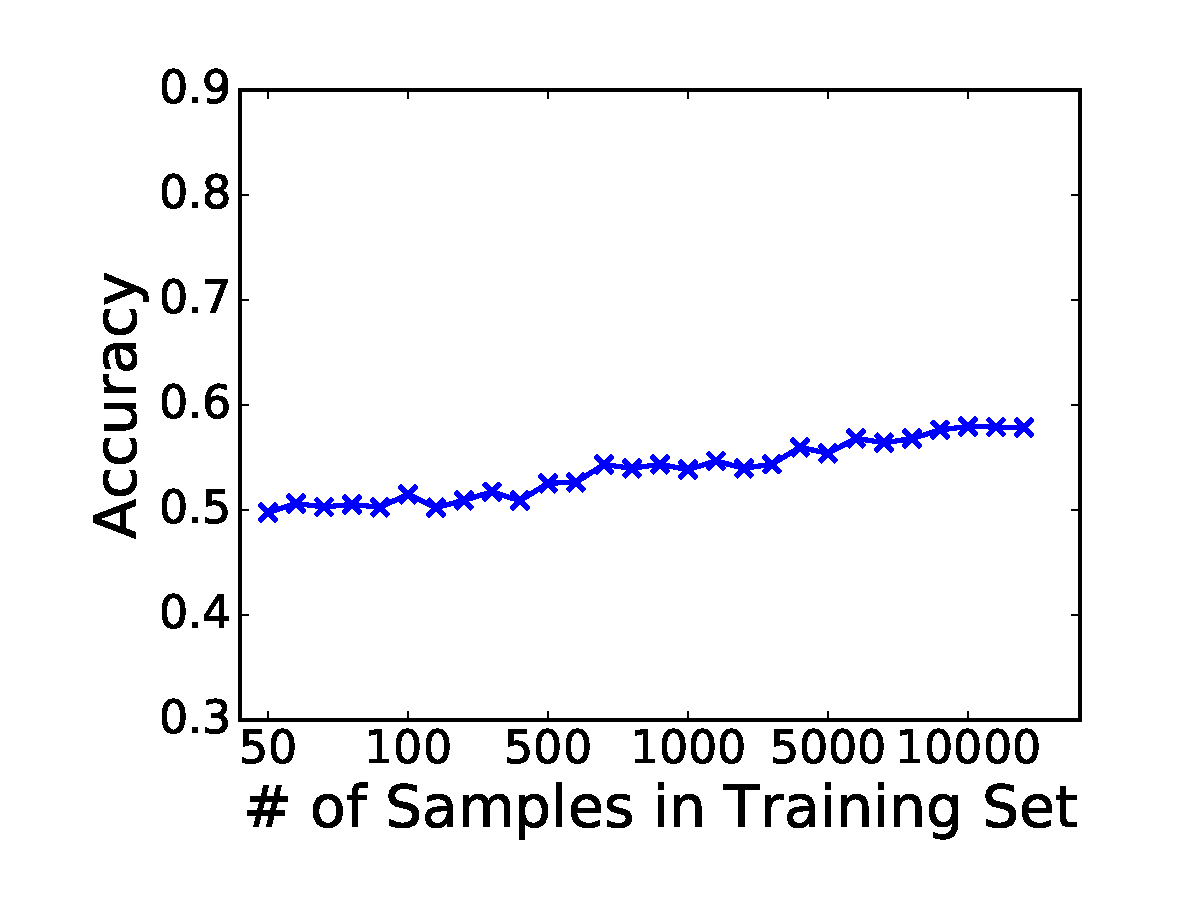
\includegraphics[width=0.16\linewidth]{figure/svm/2}\label{fig:moredata3}} 
\subfloat[Group 4]{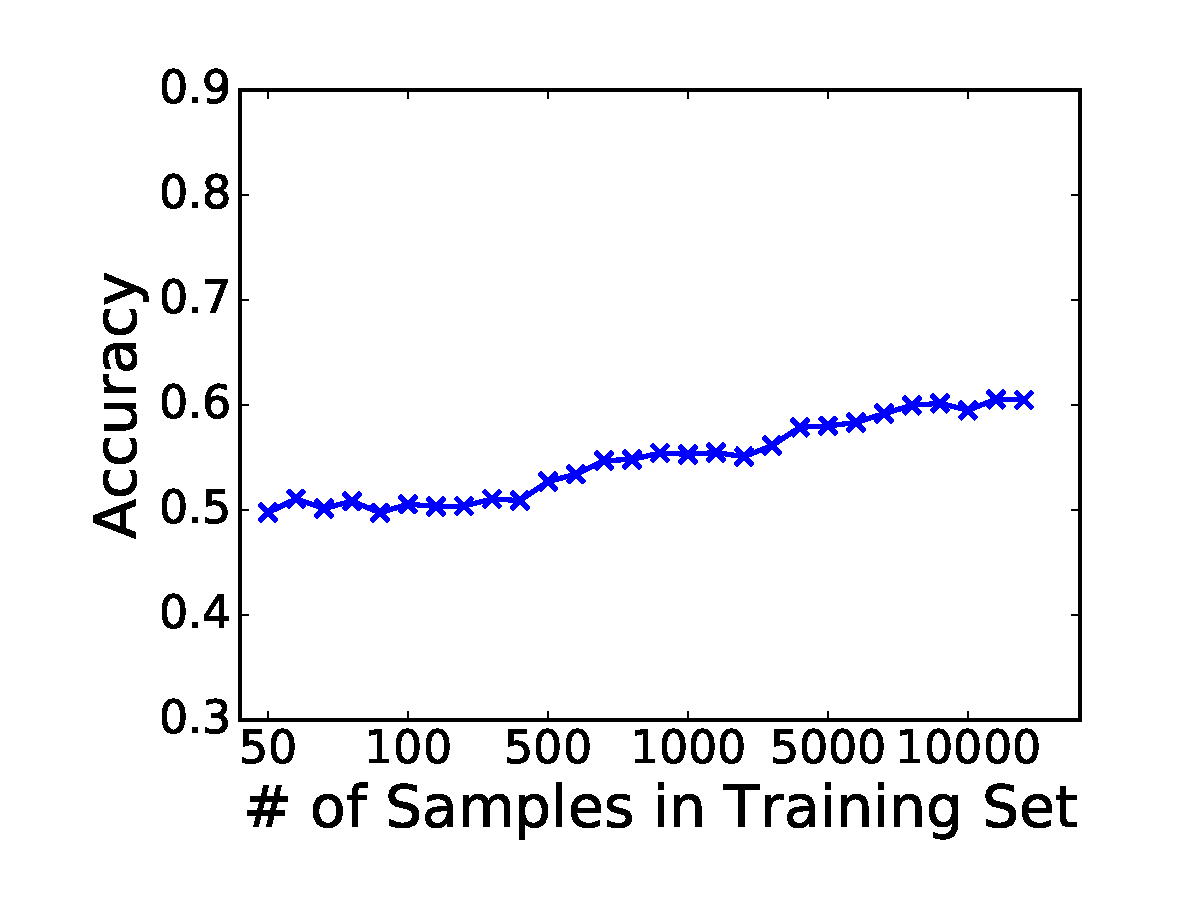
\includegraphics[width=0.16\linewidth]{figure/svm/3}\label{fig:moredata4}}
\subfloat[Group 5]{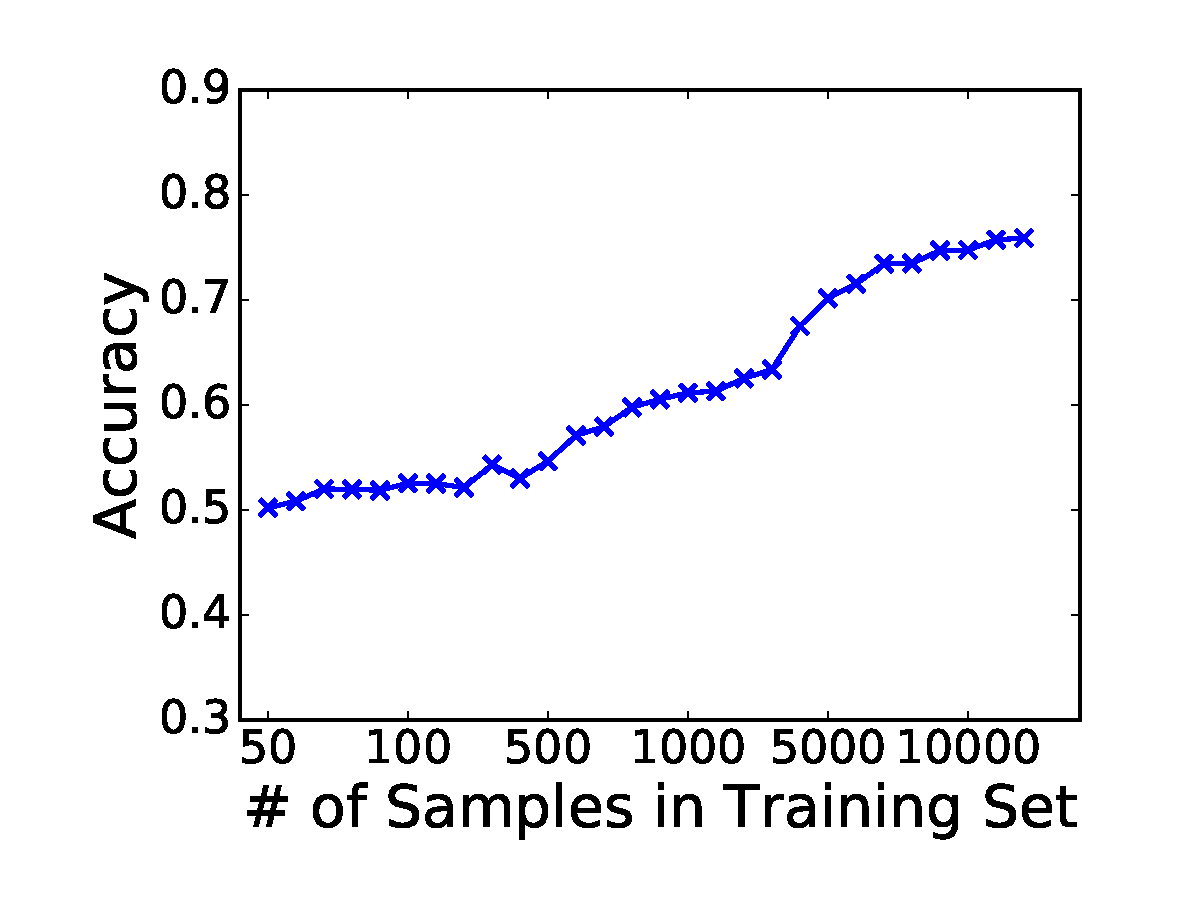
\includegraphics[width=0.16\linewidth]{figure/svm/4}\label{fig:moredata5}} \\ 

\subfloat[Group 6]{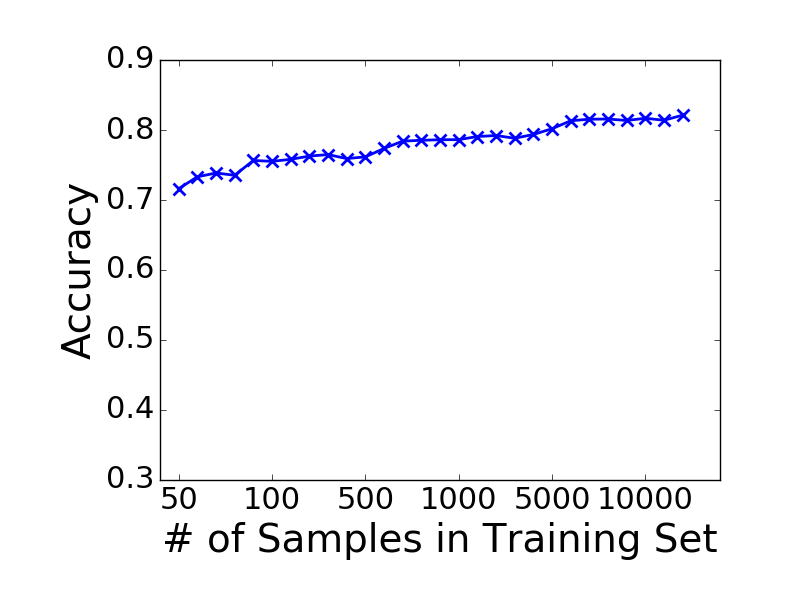
\includegraphics[width=0.16\linewidth]{figure/svm/5}\label{fig:moredata6}} 
\subfloat[Group 7]{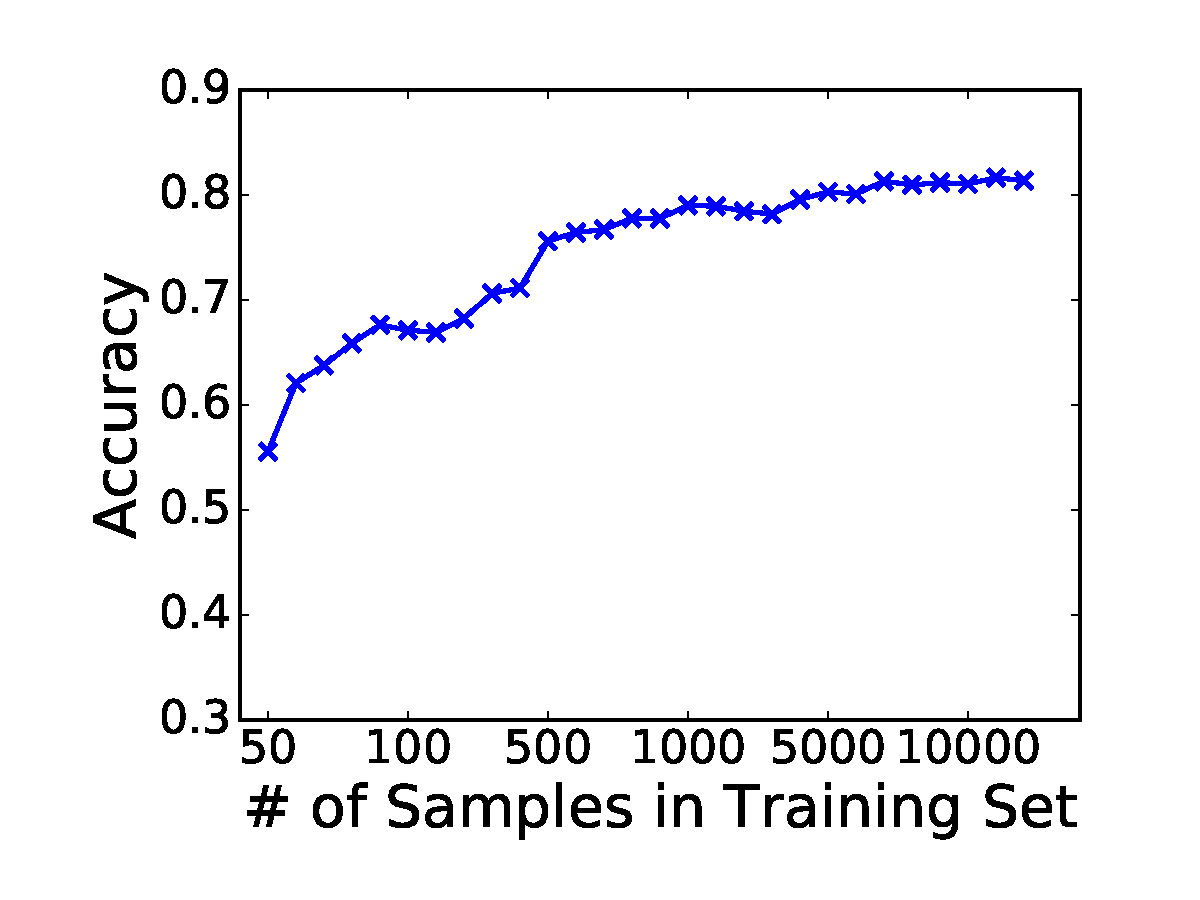
\includegraphics[width=0.16\linewidth]{figure/svm/6}\label{fig:moredata7}}
\subfloat[Group 8]{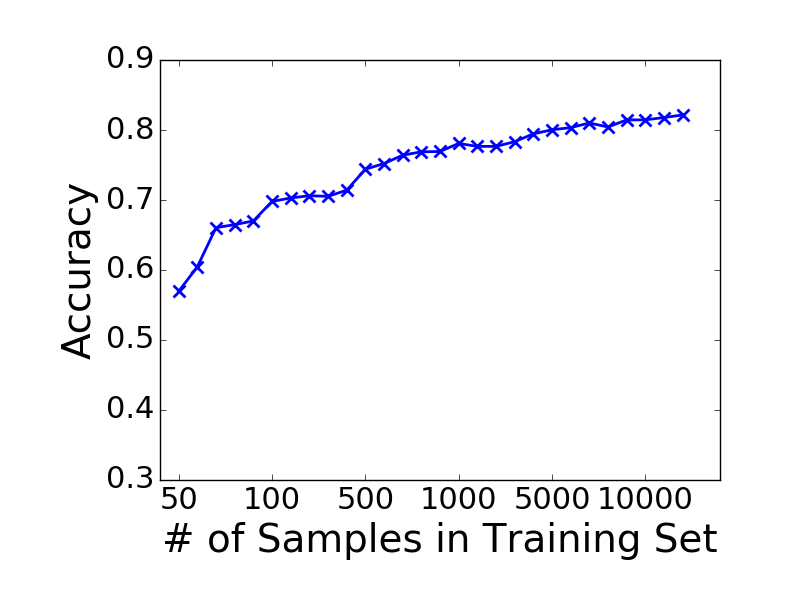
\includegraphics[width=0.16\linewidth]{figure/svm/7}\label{fig:moredata8}} 
\subfloat[Group 9]{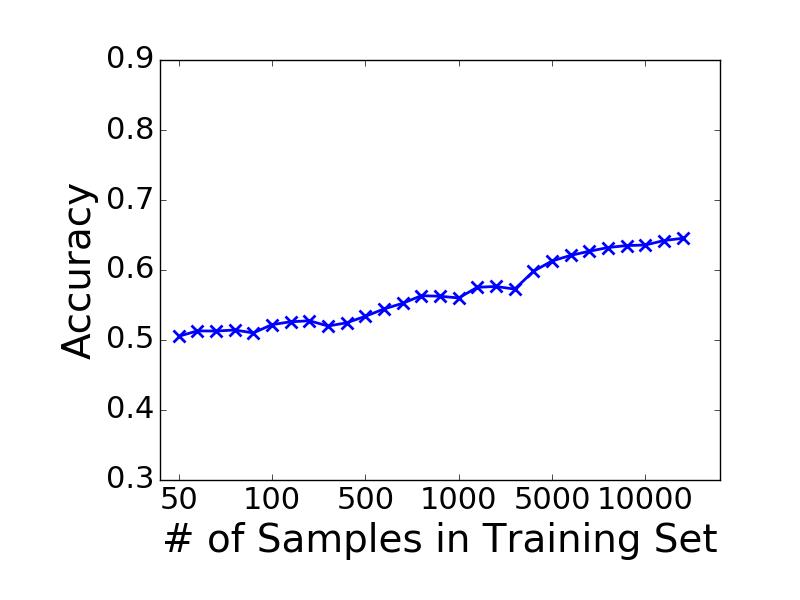
\includegraphics[width=0.16\linewidth]{figure/svm/8}\label{fig:moredata9}}
\subfloat[Group 10]{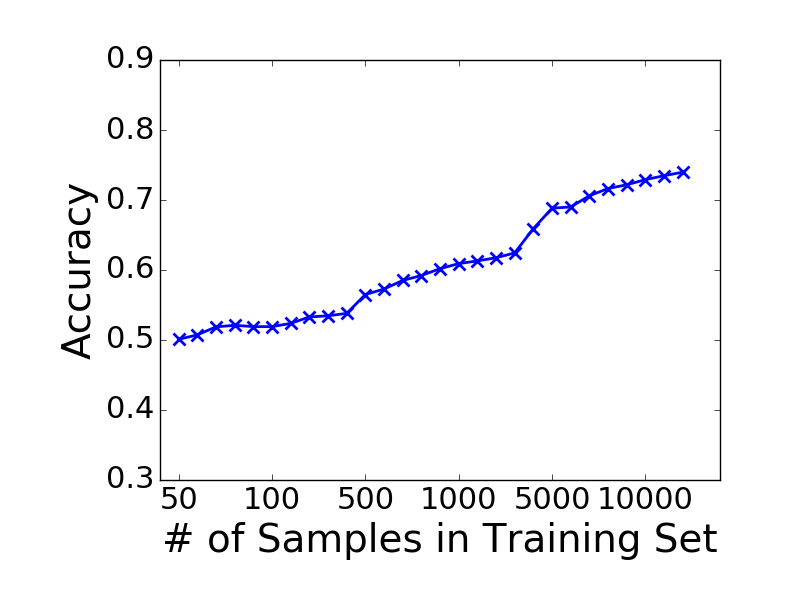
\includegraphics[width=0.16\linewidth]{figure/svm/9}\label{fig:moredata10}}
\subfloat[10-class]{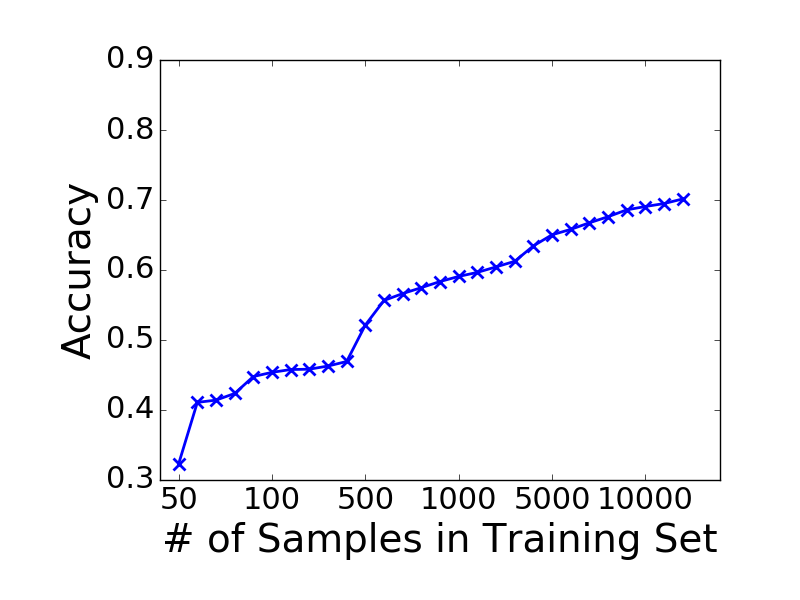
\includegraphics[width=0.16\linewidth]{figure/svm/10}\label{fig:moredata11}}
\caption{How accuracy changes with more data in traning set. 
{\footnotesize{(Figure~\ref{fig:moredata1} - Figure~\ref{fig:moredata10} show how accuracy of each two-class classifier changes 
with the size of training set changing from 50 to 10000. 
Figure~\ref{fig:moredata11} shows how accuracy of the ten-class classifier changes with the size of training set increaing from 50 to 10000. )}}} 
\label{fig:moredata} 
\end{figure*} 

%\subsection{Classification Experiments}


\subsection{Discussion}
1. Future work about indexing ssdeep string
2. Upper bound
3. More data better results
4. Need human effort or dynamic information 
\section{Related Works}
\label{sec:related}

\subsection{Leveraging Source Code Repositories}

Recently, there have been many works on exploring how to leverage open-source code repositories that contain vast amount of source code projects, 
such as GitHub, BitBucket, and CodePlex. 
SLANG~\cite{code-completion} trains statistical models using extracted sequences of API calls from large code bases
and applies the trained models to fill uncompleted programs with call innovations. 
JSNICE~\cite{big-predicting} aims to predict identifier types and obfuscated identifier names for JavaScript programs. 
A score function based on learned CRF model is optimized to make all predictions. 
Phrase-based statistical translation approaches have also been proposed
to translate C\# programs to Java programs~\cite{big-translation}. 

These systems analyze source codes by leveraging large code bases in open-source code repositories.
We have different objectives and methods: 
we analyze malwares and anti-virus engines by leveraging an open malware repository.
%and we rely on malwares’ metadata information and ssdeep hash strings calculated from binary executables.


\subsection{Analyzing and Leveraging VirusTotal}
We are not the first to investigate \vt.
The research community starts to pay more attention to VirusTotal repository recently
and there have been several works on \vt.

The closest relaed work is a recent study on \vt{}~\cite{SongAPsys2016}. 
Similar to our work, they downloaded one-month data from VirusTotal
and focused on PE files.
They studied a set of basic properties of PE malwares,
including size distribution, malware family distribution, and temporal properties.   
We collected a longer period of data from \vt.
More important, we performed deeper analysis into what are the fundamental factors 
that correlate and influence malware detection.
Apart from studying malwares, we also study anti-virus engines and how they influence each other
and perform classification and clustering on \vt\ data.
These findings provide far more insights than the previous work and will be able to help future researchers more.
%Different from our work, 
Finally, the previous work only relied on detection results from Microsoft anti-virus engines,
while we conducted our study using all engines.
%study correlations between metadata and detection results from all engines, 
%and we also evaluate different detection engines by modeling influence among different engines.  

Recently, researchers noticed that some malware writers use VirusTotal as testing platform~\cite{huangvt2016bigdata, neeles}.
They explored this phenomenon and developed techniques to identify malware writers. 
Huang \etal\ downloaded four months of VirusTotal metadata to identify Android malware development cases~\cite{huangvt2016bigdata}. 
Their technique first alerts suspicious source IDs 
and then conducts program analysis to further validate whether 
these source IDs are really testing their Android malware prototypes on \vt{}. 
Graziano \etal\ tried to identify Windows malware development cases on Anubis~\cite{neeles}. 
They used data on VirusTotal to validate their findings. 
{\color{red} Their works target to identify suspicious source IDs, 
while we focus on understanding correlations between source IDs' history and detection rate of their submissions.} 
%Their works focus on submission history of each source ID, 
%while we \yiying{fill}.  

Kantchelian \etal\ applied various supervised and unsupervised 
techniques to aggregate various labels from different anti-virus engines into one ground truth label 
on a dataset collected from VirusTotal~\cite{betterGT}. 
Their goal is to find better ground truth label for distinct samples, 
while our work tries to model influence among different anti-virus vendors.  

%3. Code classification and clustering


\section{Conclusion}
\label{sec:con}

\vt{} serves as a fruitful resource to understand malwares and anti-virus engines in the real world. 
In this paper, 
we conduct a thorough study on four months of \vt\ submission metadata.
We first study which factors correlate to submissions' detection rate 
and identified three factors: file size, submission history, and submitter reputation.
We then investigate the influence between different vendors using a graph model borrowed from the social media analysis area. 
Our experimental results show that   
%influence models borrowed from social media analysis can help predict the temporal behavior of malware detection, 
some vendors are highly influenced by all other vendors
and cautions should be taken to use these detection results.
Finally, we study whether hash strings of files are enough to build accurate machine learning classifiers and predictors. 
We design several classifiers based on ssdeep similarity and these classifiers have varied accuracy. 
We also identify a simple metric that can predict accuracy for a given classification
task.


\bibliographystyle{ACM-Reference-Format}
\bibliography{security}

\end{document}
